\documentclass{article}
\usepackage[a4paper, total={6.5in, 10in}]{geometry}
\usepackage[utf8]{inputenc}
\usepackage[english]{babel}
\usepackage{amsmath}
\usepackage{amssymb}
\usepackage{verbatim}
\usepackage{paralist}
\usepackage{xcolor}
\usepackage{tkz-euclide}
\usetkzobj{all}
\usepackage{changepage}
\usepackage{setspace}
\usetikzlibrary{arrows,automata,positioning}
\title{\textbf{Stackelberg Mean-payoff Games with One epsilon-optimal Adversarial Follower}}
\author{}
\date{February 2020}
\usepackage{amsthm}
\onehalfspace
\usepackage{cleveref}% http://ctan.org/pkg/cleveref
\usepackage{lipsum}% http://ctan.org/pkg/lipsum
\usepackage[mathlines]{lineno}
\setlength\linenumbersep{0.5cm}
\renewcommand\thelinenumber{\color{red!80!black}\arabic{linenumber}~}
\let\oldqed\qed
\renewcommand\qed{\mbox{}\hfill$\oldqed$}
\newcommand*\patchAmsMathEnvironmentForLineno[1]{%
  \expandafter\let\csname old#1\expandafter\endcsname\csname #1\endcsname
  \expandafter\let\csname oldend#1\expandafter\endcsname\csname end#1\endcsname
  \renewenvironment{#1}%
  {\linenomath\csname old#1\endcsname}%
  {\csname oldend#1\endcsname\endlinenomath}}% 
\newcommand*\patchBothAmsMathEnvironmentsForLineno[1]{%
  \patchAmsMathEnvironmentForLineno{#1}%
  \patchAmsMathEnvironmentForLineno{#1*}}%
\AtBeginDocument{%
  \patchBothAmsMathEnvironmentsForLineno{equation}%
  \patchBothAmsMathEnvironmentsForLineno{align}%
  \patchBothAmsMathEnvironmentsForLineno{flalign}%
  \patchBothAmsMathEnvironmentsForLineno{alignat}%
  \patchBothAmsMathEnvironmentsForLineno{gather}%
  \patchBothAmsMathEnvironmentsForLineno{multline}%
}
\linenumbers
\newtheorem{theorem}{Theorem}[section]
\newtheorem{corollary}[theorem]{Corollary}
\newtheorem{lemma}[theorem]{Lemma}
\newtheorem{conjecture}[theorem]{Conjecture}
\newtheorem{definition}[theorem]{Definition}
\newtheorem{proposition}[theorem]{Proposition}
\newtheorem{remark}[theorem]{Remark}
\newtheorem{example}[theorem]{Example}
\crefname{lemma}{Lemma}{Lemmas}
\crefname{remark}{Remark}{Remarks}
\crefname{theorem}{Theorem}{Theorems}
\crefname{conjecture}{Conjecture}{Conjectures}
\crefname{corollary}{Corollary}{Corollaries}
\crefname{proposition}{Proposition}{Propositions}
\crefname{figure}{Figure}{Figures}
\crefname{example}{Example}{Examples}

\newcounter{casenum}
\newenvironment{caseof}{\setcounter{casenum}{1}}{\vskip.5\baselineskip}
\newcommand{\case}[2]{\vskip.5\baselineskip\par\noindent {\bfseries Case \arabic{casenum}:} #1\\#2\addtocounter{casenum}{1}}
\newcommand{\track}[1]{{\textcolor{red}{#1}}}
\newcommand{\nat}{{\mathbb{N}}}
\newcommand{\sgcomment}[1]{{\footnotesize \color{purple}[#1 - \textbf{Shibashis}]}}
\newcommand{\mbcomment}[1]{{\footnotesize \color{blue}[#1 - \textbf{Mrudula}]}}

\begin{document}
\maketitle

\section{Introduction} 
  \label{sec:intro}
  % \sgcomment{We write here about 
% \begin{enumerate}
%     \item Stackelberg games including history (Refer to 1934 paper by Stackelberg); comparison with Nash equilibrium and state that Stackelberg strategy may produce greater payoff for the leader than in the Nash equilibrium.
%     \item application of Stackelberg games
% \end{enumerate}}

Stackelberg games were introduced by German economist Heinrich Freiherr von Stackelberg in \cite{S34} to simulate how firms behave in the market. The players of this game comprise of one leader firm and multiple follower firms. The leader starts the game by announcing her strategy and the followers respond by playing the optimal response to the leader's strategy.

Stackelberg Games have been studied for Bi-Matrix games \cite{GS18}. A well-known notion of equilibrium is the Nash equilibrium (NE) \cite{Nash50}, which is a profile of strategies for each player such that no player can deviate from her current strategy in the profile unilaterally, and thereby get benefited.

\begin{table}[]
    \centering
    \begin{tabular}{ll|c|c|}
        \cline{3-4}
        & & \multicolumn{2}{c|}{Follower} \\ 
        \cline{3-4} 
        & & I & II \\ 
        \hline
        \multicolumn{1}{|c|}{\multirow{2}{*}{Leader}} & \multicolumn{1}{c|}{I}  & (1, 4) & (4, 2)\\ 
        \cline{2-4} 
        \multicolumn{1}{|c|}{} & \multicolumn{1}{c|}{II} & (1, 3) & (3, 5) \\
        \hline
    \end{tabular}
    \caption{Example of Nash vs Stackelberg Equilibrium in a bi-matrix game}
    \label{tab:bi-matrix-game}
\end{table}

We demonstrate here with a classical bi-matrix game shown in \cref{tab:bi-matrix-game} how the power to communicate her strategy would help the leader achieve a better payoff than what she can get in an NE. Considering pure strategy profiles, the only pure strategy Nash equilibrium is the profile (I, I). It gives a payoff of 1 to the leader and a payoff of 4 to the follower. However, if the leader announces that she will play strategy II, the best response for the follower is to play strategy II as it gives him the highest payoff. A leader strategy profile \cite{GS18} is one for which the follower cannot make a beneficial deviation. We call a profile to be a Stackelberg Equilibrium that gives the leader the maximal payoff among all the leader strategy profiles. Thus, the strategy profile (II, II) is a Stackelberg equilibrium and gives the leader a payoff of 3.

% Let us demonstrate why Stackelberg Equilibria produce a better payoff than their Nash counterparts with an example. Consider the period of 1894 - 1999 where the motorcycle manufacturers were in a competition to produce the fastest production motorcycle. After over a century of one-upmanship, some regulators and politicians in Europe, fearing an outbreak of illegal racing as riders try to break the 200 mph barrier, called for an import ban against high speed motorcycles. To preempt regulation and avoid negative publicity, the manufacturers voluntarily entered into a \text{Gentlemen's agreement} to limit the speed of their machines to 300 kmph (186 mph), starting with 2000 models. A Nash Equilibrium strategy would suggest that each company must break the agreement to produce a faster motorcycle, thus getting a higher market share. But breaking the agreement would likely result in an import ban regulation which would imply a huge market loss for all manufacturers involved. On the other hand, a Stackelberg Equilibrium strategy would explain why that no company must break the agreement, and thus would ideally yield equal market share for all motorcycle companies involved.\cite{WIKI00}

\begin{figure}
    \centering
    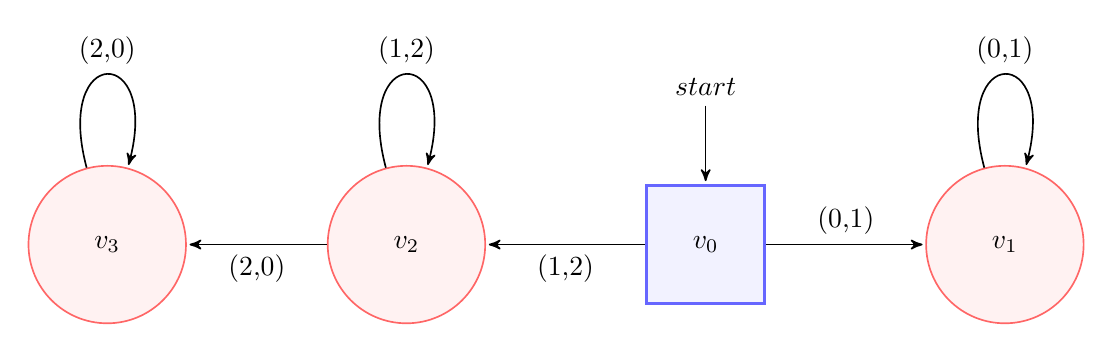
\begin{tikzpicture}[->,>=stealth',shorten >=1pt,auto,node distance=3.8cm,
                        semithick, squarednode/.style={rectangle, draw=blue!60, fill=blue!5, very thick, minimum size=15mm}]
      \tikzstyle{every state}=[fill=white,draw=black,text=black,minimum size=2cm]
    
      \node[squarednode]                                                 (A)              {$v_0$};
      \node[state, draw=red!60, fill=red!5]                              (B) [left of=A]  {$v_2$};
      \node[state, draw=red!60, fill=red!5]                              (C) [right of=A] {$v_1$};
      \node[draw=none, fill=none, minimum size=0cm, node distance = 2cm] (D) [above of=A] {$start$};
      \node[state, draw=red!60, fill=red!5]                              (E) [left of=B]  {$v_3$};
      \path (A) edge              node {(1,2)} (B)
                edge              node {(0,1)} (C)
            (B) edge [loop above] node {(1,2)} (B)
                edge              node {(2,0)} (E)
            (C) edge [loop above] node {(0,1)} (C)
            (E) edge [loop above] node {(2,0)} (E)
            (D) edge [left] node {} (A);
    \end{tikzpicture}
    \caption{An example in which Stackelberg equilibrium for Player $0$ gives better payoff than Nash equilibrium.}
    \label{fig:nash_vs_stackelberg}
\end{figure}

We also give another example involving a mean-payoff game showing that the Stackelberg Equilibrium may produce a better payoff for the leader than all Nash equilibria. Consider the example depicted in \cref{fig:nash_vs_stackelberg}. There are two players: we call them the leader and the follower. The leader owns the circle vertices and the square vertices are owned by the follower. We consider only pure strategies for each player. Now, consider the strategy $\sigma_L^{\mathsf{Nash}}$ of the leader in which she plays $v_1 \to v_1$, $v_2 \to v_3$ and $v_3 \to v_3$. Let $\sigma_F^{\mathsf{Nash}}$ be a strategy of the follower in which he plays $v_0 \to v_1$. Clearly, the strategy profile ($\sigma_L^{\mathsf{Nash}}$, $\sigma_F^{\mathsf{Nash}}$) is a Nash Equilibrium that yields a payoff of 0 to the leader. However, if the leader announces a strategy $\sigma_L^{\mathsf{Stackelberg}}$ where she plays $v_1 \to v_1$, $v_2 \to v_2$ and $v_3 \to v_3$, the follower will get a better payoff if he responds with a strategy $\sigma_F^{\mathsf{Stackelberg}}$ where he plays $v_0 \to v_2$. Thus, the strategy profile ($\sigma_L^{\mathsf{Stackelberg}}$, $\sigma_F^{\mathsf{Stackelberg}}$) is a Stackelberg Equilibrium and yields a payoff of 1 for the leader.

\begin{figure}
    \centering
    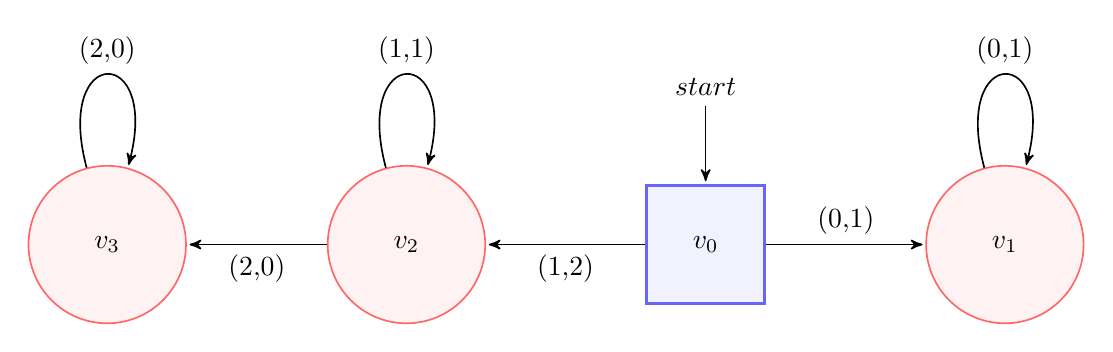
\begin{tikzpicture}[->,>=stealth',shorten >=1pt,auto,node distance=3.8cm,
                        semithick, squarednode/.style={rectangle, draw=blue!60, fill=blue!5, very thick, minimum size=15mm}]
      \tikzstyle{every state}=[fill=white,draw=black,text=black,minimum size=2cm]
    
      \node[squarednode]                                                 (A)              {$v_0$};
      \node[state, draw=red!60, fill=red!5]                              (B) [left of=A]  {$v_2$};
      \node[state, draw=red!60, fill=red!5]                              (C) [right of=A] {$v_1$};
      \node[draw=none, fill=none, minimum size=0cm, node distance = 2cm] (D) [above of=A] {$start$};
      \node[state, draw=red!60, fill=red!5]                              (E) [left of=B]  {$v_3$};
      \path (A) edge              node {(1,2)} (B)
                edge              node {(0,1)} (C)
            (B) edge [loop above] node {(1,1)} (B)
                edge              node {(2,0)} (E)
            (C) edge [loop above] node {(0,1)} (C)
            (E) edge [loop above] node {(2,0)} (E)
            (D) edge [left] node {} (A);
    \end{tikzpicture}
    \caption{Co-operative Stackelberg Equilibrium vs Adversarial Stackelberg Equilibrium}
    \label{fig:co-operative_vs_adversarial}
\end{figure}

Thus, we can see that the leader with the power to communicate her strategy can influence the follower to play a strategy which she desires and thereby get a better payoff for herself. Both the leader and the follower aim at maximising their respective payoffs. However, the follower can have multiple optimal responses to the leader's strategy. Two different scenarios can be considered in this setting: either the optimal-response strategy is imposed by the leader (or equivalently chosen co-operatively by the two players), or the optimal-response strategy is chosen adversarially by the follower. We demonstrate the two scenarios with an example depicted in \cref{fig:co-operative_vs_adversarial}. Here, the leader can announce her strategy $\sigma_L$ where she plays $v_2 \to v_2$. However, in this example the follower has two optimal responses, i.e. he can play $v_0 \to v_1$ or $v_0 \to v_2$. If the follower is co-operative, then he will choose the strategy which also maximises the leader's payoff. In this example, the co-operative follower will choose to play the strategy $v_0 \to v_2$. Thus, in the co-operative setting, the leader receives a payoff of 1 and the follower receives a payoff of 1. But if the follower is adversarial, he will choose the strategy which minimises the payoff of the leader. In this example, the adversarial follower will choose to play $v_0 \to v_1$. Thus, in the co-operative setting, the leader receives a payoff of 0 and the follower receives a payoff of 1.

The adversarial case is more interesting because it allows us to model the situation in which the leader can only choose her strategy and must be prepared to face any rational response of follower, i.e. if follower has several possible optimal responses then the leader's strategy should be designed to face all of them.

In this work, we study the notion of Adversarial Stackelberg Equilibria on two-player non-zero sum infinite duration mean-payoff games played on graph arenas. Here, the two players are the leader, also called Player~0 and the follower, also called Player~1. The game comes with two (usually $\mathbb{R}$-valued) mean-payoff functions that determine the payoff each player receives. As mentioned before, in a Stackelberg game, players play sequentially as follows.
\begin{inparaenum}[(i)]
\item Player~0, the leader, announces her choice of strategy $\sigma_0$. 
\item Player~1, the follower, announces his choice of strategy $\sigma_1$ in response to the leader's strategy $\sigma_0$. 
\item Both players receive their respective mean-payoffs determined by their respective mean-payoff functions.
\end{inparaenum}
Due to the sequential nature of the game, Player~1 knows the strategy $\sigma_0$, and so to act rationally he should choose a strategy that maximises his payoff. If such a strategy exists, it is called a best-response to Player~0's strategy $\sigma_0$. However, best-responses are not guaranteed to always exist \cite{FGR20}. Thus, the authors of \cite{FGR20} consider the notion of $\epsilon$-optimal best responses. Here, the follower, i.e., Player~1  plays any strategy that gives him a payoff that is up to an $\epsilon$ amount lesser than the best payoff he can receive. In \cite{FGR20}, it is  established that for every $\epsilon > 0$, there always exists an $\epsilon$-optimal best response of Player~1 to every strategy of Player~0. The leader will choose, over all $\epsilon \geqslant 0$, a strategy such that the payoff she receives is as large as possible when the follower plays any adversarial $\epsilon$-optimal best response. We call the supremum of payoffs obtained by the leader over all possible $\epsilon$ values when she plays such a strategy as the Adversarial Stackelberg Value, or simply, the $\mathbf{ASV}$.

In this work, we assume that Player~1 is not completely rational, and hence Player~1 would always choose an $\epsilon$-optimal best-response to Player~0's strategy $\sigma_0$, i.e., we fix the value of $\epsilon$ \emph{a priori}.
In turn, if the leader assumes an almost-rational response of the follower to her strategy, this should guide the leader when choosing her strategy $\sigma_0$. Indeed, the leader should choose a strategy $\sigma_0 $ such that payoff she receives is as large as possible when the follower plays an adversarial $\epsilon$-optimal best-response, for a fixed $\epsilon$. We call the payoff obtained by the leader when she plays such a strategy as the $\epsilon$-optimal Adversarial Stackelberg Value, or simply, the $\mathbf{ASV}^{\epsilon}$.

\textbf{\bf Our contribution}

\begin{table}[]
\centering
\begin{tabular}{|c|c|c|c|}
\hline
 &
  Threshold Problem &
  Computing ASV &
  Achievability \\ \hline
\begin{tabular}[c]{@{}c@{}}Adversarial \\ Follower\end{tabular} &
  \begin{tabular}[c]{@{}c@{}}{\color[HTML]{009901} NP-Time} \\ \\ {\color[HTML]{0000FE} \textbf{Finite Memory}} \\ {\color[HTML]{0000FE} \textbf{Strategy [\cref{LemFinMemWitnessASVNonEps}]}} \end{tabular} &
  {\color[HTML]{009901} Theory Of Reals} &
  {\color[HTML]{009901} No} \\ \hline
\begin{tabular}[c]{@{}c@{}}Adversarial\\ Epsilon-Optimal \\ Follower\end{tabular} &
  {\color[HTML]{0000FE} \textbf{\begin{tabular}[c]{@{}c@{}}NP-Time\\ \\ Finite Memory \\ Strategy [\cref{ThmNpForASV}] \end{tabular}}} &
  {\color[HTML]{0000FE} \textbf{\begin{tabular}[c]{@{}c@{}}Theory Of Reals [\cref{ThmComputeASV}]/\\ \\ Solving LP \\ in EXP-Time [\cref{ExpTimeForComputeASV}]\end{tabular}}} &
  {\color[HTML]{0000FE} \textbf{\begin{tabular}[c]{@{}c@{}}Yes [\cref{ConjAchiev}]\\ \\ (Requires Infinite \\ Memory [\cref{ThmExNeedInfMem}])\end{tabular}}} \\ \hline
\end{tabular}
\caption{
    {\color[HTML]{0000FE} \textbf{Results obtained in our work are in blue and in bold-text }} whereas {\color[HTML]{009901} results obtained in \cite{FGR20} are in green and in normal-text}
}
\label{tab:results}
\end{table}

\track{This work is an extension of the work done in \cite{FGR20}. The authors in \cite{FGR20} assume that the follower is rational and will always play an adversarial best response for a given strategy of leader. In this work, we assume that the follower is almost rational and will always play an $\epsilon$-optimal adversarial best response to the strategy of the leader, for a fixed $\epsilon > 0$. This has produced results which are described below and also summarized in \cref{tab:results}.}

We begin by showing that infinite memory is required for Player~0 to achieve the $\mathbf{ASV}^{\epsilon}$ [\cref{ThmExNeedInfMem}]. A similar result is shown in \cite{FGR20} in which the leader, Player~0, needs infinite memory to achieve $\mathbf{ASV}$.

We also consider the memory required by Player~1 to play $\epsilon$-optimal best responses to a strategy of Player~0. We show that Player~1 may require infinite memory to play an $\epsilon$-optimal best-response [\cref{ThmP1NeedInfMem}]. \track{We do this by describing a mean-payoff game where for a given strategy of Player~0, no finite memory strategy of Player~1 is sufficient to play an $\epsilon$-optimal best response.} Indeed, we show that there does not exist an $\epsilon$-optimal best response that uses finite memory.

Recall that for a given mean-payoff game and a rational value $c$, the threshold problem is to as check if $\mathbf{ASV}^{\epsilon} > c$. Similar to the results obtained in \cite{FGR20}, we introduce a notion of $\epsilon$-witness for proving that $\mathbf{ASV}^{\epsilon} > c$ [\cref{ThmWitnessASVInfMem}]. But here, we go a step further by developing a finite memory strategy for Player~0 to achieve this $\mathbf{ASV}^{\epsilon}$ threshold value. This finite memory strategy can be synthesised in $\mathsf{NP}$-time [\cref{ThmNpForASV}]. Additionally, we prove that a finite memory strategy is sufficient to achieve $\mathbf{ASV} > c$ [\cref{LemFinMemWitnessASVNonEps}]. Besides, our proof for the existence of an $\epsilon$-witness uses techniques that are very different from the ones used in \cite{FGR20}.

We explore the effect of limiting Player~0's memory on the Adversarial Stackelberg Value. We define $\mathbf{ASV}^{\epsilon}_{\mathsf{FM}}$ as the Adversarial Stackelberg Value obtained by Player~0 when she is limited to playing only finite memory strategies. In this work, we show that $\mathbf{ASV}^{\epsilon}_{\mathsf{FM}} = \mathbf{ASV}^{\epsilon}$, i.e., the finite memory constraint has no effect on the Adversarial Stackelberg Value [\cref{CorASVEqASVFin}].

Next we study the problem of computation of $\mathbf{ASV}^{\epsilon}$. In \cite{FGR20}, it has been established that the $\mathbf{ASV}$ can be expressed as a formula in the theory of reals with addition, and can be computed with quantifier elimination. However, no precise complexity results have been provided. In this work, we show that we can adapt the methods used in \cite{FGR20} to express the $\mathbf{ASV}^{\epsilon}$ as a formula in the theory of reals with addition [\cref{ThmComputeASV}]. Further, this approach of using theory of reals with addition gives us the necessary intuition to formulate the problem of computing $\mathbf{ASV}^{\epsilon}$ using a set of linear programs, where each linear program has exponential number of constraints, thus giving us a $\mathsf{EXP}$-time algorithm to compute the $\mathbf{ASV}^{\epsilon}$ [\cref{ExpTimeForComputeASV}]. 

Finally, we study the problem of achievability of $\mathbf{ASV}^{\epsilon}$. The $\mathbf{ASV}^{\epsilon}$ is said to be achievable if there exists a strategy $\sigma_0$ for Player~0 such that Player~0 by choosing the strategy $\sigma_0$ receives a payoff that is greater than or equal to the $\mathbf{ASV}^{\epsilon}$. While in \cite{FGR20}, it has been shown that $\mathbf{ASV}$ is not always achievable, here, in contrast to the results obtained in \cite{FGR20}, we show that $\mathbf{ASV}^{\epsilon}$ is always achievable [\cref{ConjAchiev}].

\textbf{Related Work} In \cite{FKL10}, the authors introduce the notion of rational synthesis in the co-operative setting for omega-regular objectives. Here, the game is defined as having one system player and a set of n players, also known as agents. Each player has a temporal objective. For a given solution concept, the problem of rational synthesis is to return an outcome of the game that satisfies the objective of the system player and a strategy profile for the set of n agents that is a solution in the game with respect to the solution concept. Three main solution concepts are studied in this work: dominant strategy, Nash equilibrium and subgame perfect equilibrium. 

In \cite{KPV16}, the authors study the notion of adversarial rational synthesis. Contrary to the assumption in \cite{FKL10}, the authors in \cite{KPV16} assume that the agents will not follow the strategy assigned to them in the strategy profiles for the different solution concepts. For a given solution concept, the problem of adversarial rational synthesis is to return an outcome that satisfies the objective of the system player for every strategy profile for the set of n agents that is a solution in the game with respect to the solution concept. Here, the two solution concepts which are studied are: dominant strategy and nash equilibrium.

In \cite{CFGR16}, the authors study the notion of co-operative and adversarial rational synthesis where the players in the game have various omega-regular objectives such as safety, reachability, parity, etc. The complexity results for the various objectives are established in both the adversarial and co-operative setting. 

In \cite{GS14}, the authors study multi-player mean-payoff Stackelberg games in the co-operative setting. In this work, the multi-player mean-payoff games have one leader player and multiple stackelberg players. The authors also provide a polynomial time reduction from multi-player setting to a two-player setting.

In \cite{GS18}, the authors study both Stackelberg (leader) equilibrium and incentive equilibrium over bi-matrix games. It is not difficult to see that the leader can improve upon her payoff by providing an incentive to her follower which is actually a share of her own payoff. They define the leader strategy profile as one in which the follower cannot improve his payoff by deviating, and hence every Nash equlibrium is a leader strategy profile. A Stackelberg or leader equilibrium is a leader strategy profile that gives the highest payoff to the leader. Every leader strategy profile is an incentive strategy profile with incentive value $0$. Since in this work, the authors consider mixed strategies, the existence of Nash equilibrium in bi-matrix games \cite{Nash50,LH64} implies the existence of leader and incentive equilibria.

In \cite{GSTDP16}, the authors study the concept of Incentive Stackelberg mean-payoff games, where in addition to assigning strategies to all players, the leader can also transfer parts of her payoff to other players and incentivise them to follow the assigned strategy. This ability to incentivise her followers provides the leader with more freedom in selecting strategy profiles, and thus can improve the payoff for the leader in such games even when compared with Stackelberg equilibrium.

In \cite{CHJ06}, the authors study secure Nash equilibrium, where the objectives are considered in a lexicographic order. The two players try to first maximise their own payoffs, and then minimize the payoff of the other player. A secure Nash equilibrium is a Nash equilibrium. 

In \cite{PFKSV14}, the authors study Secure Equilibrium in multi-player games in two different settings: 
\begin{inparaenum}[(i)]
    \item In the first setting, the games have probabilistic transitions, i.e. the play moves from one state to another state according to a probability measure, which may depend on the current state and the chosen action of the player who owns the state. The games in this setting have bounded and continuous payoff functions.
    \item In the second setting, the games have deterministic transitions. The games in this setting have qualitative Borel payoff functions.
\end{inparaenum}

In \cite{GS15}, the authors study the effects of limited memory on both Nash and Stackelberg(or Leader) Equilibria in Multi-player discounted sum games. In this work, there exists one powerful player (leader) with the ability to select the strategies of all players for Nash and Leader equilibria, where in Leader equilibria the Nash condition is waived for the strategy of this powerful player.

In \cite{FGR20}, the authors study Stackelberg mean-payoff Games in adversarial setting and  Stackelberg discounted sum games in both adversarial and co-operative setting.

\textbf{Application of Adversarial Stackelberg games} Adversarial Stackelberg games can be relevant in several contexts. Consider two belligerent countries, say $A$ and $B$ that are engaged in increasing their nuclear arsenal. There may be a country, let's say $A$ that is more powerful than the other. While both the countries are under mutual threat, however it is likely that the less powerful country gets more seriously affected in the case of a war. So it is in the interest of the more powerful country to attack the less powerful one. On the other hand, any attack from the more powerful country $A$ may lead the country $B$ to stop exporting to $A$ some goods that are of high value to $A$. The resultant state models the situation of a Nash equilibrium. If the more powerful country, on the other hand, pledges to commit to a nuclear non-proliferation, and asks country $B$ to do the same, it may be possible that the less powerful country will also follow the same, and both the countries save expenses on increasing their nuclear arsenal. However, since the less powerful country $B$ does not have a cordial relation with country $A$, it will try to act in a way that harms  country $A$ whenever possible modelling the case of an Adversarial Stackelberg game.

In \cite{GS18}, the authors consider a class of Arms Race game as an example for incentive equilibrium.


% \sgcomment{{\bf Related Work} We should look at the following papers:
% \begin{enumerate}
%     \item Dana Fisman, Orna Kupferman, and Yoad Lustig. Rational synthesis. (Even these papers possibly talk about the co-operative setting, and not the adversarial setting.)
%     \item Orna Kupferman, Giuseppe Perelli, and Moshe Y. Vardi. Synthesis with rational environments.
%     \item Rodica Condurache, Emmanuel Filiot, Raffaella Gentilini, and Jean-François Raskin. The complexity of rational synthesis.
%     \item Emmanuel Filiot, Raffaella Gentilini, and Jean-François Raskin. Rational synthesis under imperfect information.
%     \item Anshul Gupta and Sven Schewe. Quantitative verification in rational environments.
%     \item Anshul Gupta, Sven Schewe. Buying Optimal Payoffs in Bi-Matrix Games
%     \item Anshul Gupta, Sven Schewe, Ashutosh Trivedi, Maram Sai Krishna Deepak, and Bharath Kumar Padarthi. Incentive stackelberg mean-payoff games.
%     \item \mbcomment{We should also look at the literature for stochastic Stackelberg games}
%     \item Krishnendu Chatterjee, Thomas A. Henzinger, Marcin Jurdzinski. Games with Secure Equilibria
%     \item Julie De Pril, János Flesch, Jeroen Kuipers, Gijs Schoenmakers, Koos Vrieze. Existence of Secure Equilibrium in Multi-player Games with Perfect Information
%     \item Anshul Gupta, Sven Schewe, and Dominik Wojtczak. Making the best of limited memory in multi-player discounted sum games
%     \item Emmanuel Filiot, Raffaella Gentilini, and Jean-François Raskin. The Adversarial Stackelberg Value in Quantitative Games
% \end{enumerate}}

\textbf{Structure of the \mydoc} In \cref{sec:prelim}, we introduce the necessary preliminaries for our definitions and developments. Here, we provide a formal description of the game setting and describe $\epsilon$-optimal best responses. We then define the $\mathbf{ASV}^{\epsilon}$. \track{Additionally, we also talk about convex hull and ${\sf F_{\min}}$.}
In \cref{sec:examples}, we examine the memory requirements of both players for playing their strategies. We establish that Player~0 may require infinite memory to achieve the $\mathbf{ASV}^{\epsilon}$ [\cref{ThmExNeedInfMem}]. We also establish that Player~1 may require infinite memory to play an $\epsilon$-optimal best response [\cref{ThmP1NeedInfMem}]. 
In \cref{sec:ThresholdProblem}, we consider the threshold problem, i.e. checking if $\mathbf{ASV}^{\epsilon} > c$. We define a notion of $\epsilon$-witness for $\mathbf{ASV}^{\epsilon} > c$ and show that $\mathbf{ASV}^{\epsilon} > c$ if and only if there exists an $\epsilon$-witness for $\mathbf{ASV}^{\epsilon} > c$ [\cref{ThmWitnessASVInfMem}]. We also define a notion of $\epsilon$-regular-witness, and construct a finite memory strategy for Player~0 in $\mathsf{NP}$-time that achieves $\mathbf{ASV}^{\epsilon} > c$ [\cref{ThmNpForASV}]. We also study the effect of limiting Player~0 to playing finite memory strategies on the $\mathbf{ASV}^{\epsilon}$ [\cref{lemWitnessASVForFinStrat}]. We define $\mathbf{ASV}^{\epsilon}_{\mathsf{FM}}$ as the adversarial Stackelberg value Player~0 receives when she is restricted to playing finite memory strategies.
In \cref{sec:ComputeASV}, we present an algorithm to compute the $\mathbf{ASV}^{\epsilon}$. We first express $\mathbf{ASV}^{\epsilon}$ as a formula in theory of reals with addition [\cref{ThmComputeASV}]. We then express this formula as a set of exponentially many linear programs, and thus show that $\mathbf{ASV}^{\epsilon}$ can be computed in $\mathsf{ExpTime}$ [\cref{ExpTimeForComputeASV}].
In \cref{sec:FMASV}, we present a memory improvement for a previous result established in \cite{FGR20}, i.e, we show the existence of finite memory strategy to achieve the threshold problem of $\mathbf{ASV} > c$ [\cref{LemFinMemWitnessASVNonEps}]. We also show that $\mathbf{ASV}^{\epsilon}_{\mathsf{FM}} = \mathbf{ASV}^{\epsilon}$ [\cref{CorASVEqASVFin}].
In \cref{sec:Achievability}, we show that the $\mathbf{ASV}^{\epsilon}$ is always achievable [\cref{ConjAchiev}].

\section{Preliminaries}
  \label{sec:prelim}
  \textbf{Arenas} An (bi-weighted) arena $\mathcal{A}=(V, E, \langle V_0, V_1 \rangle, w_0, w_1)$ consists of a finite set $V$ of vertices, a set $E \subseteq V \times V$ of edges such that for all $v \in V$ there exists $v' \in V$ such that $(v, v') \in E$, a partition $\langle V_0, V_1 \rangle$ of $V$ , where $V_0$ (resp. $V_1$) is the set of vertices for Player~0 (resp. Player~1), and two edge weight functions $w_0 : E \rightarrow Z$, $w_1 : E \rightarrow Z$. In the sequel, we denote the maximum absolute value of a weight in $\mathcal{A}$ by $W$ .
\\
\\
\noindent\textbf{Plays and histories} A play in $\mathcal{A}$ is an infinite sequence of vertices $ \pi = \pi_0\pi_1 \dots \in V^{\omega}$ such that for all $k \in \mathbb{N}$, $(\pi_k, \pi_{k+1}) \in E$. We denote by $\mathbf{Plays}_{\mathcal{A}}$ the set of plays in $\mathcal{A}$, omitting the subscript $\mathcal{A}$ when the underlying arena is clear from the context. Given $ \pi = \pi_0\pi_1\dots \in \mathbf{Plays}_{\mathcal{A}}$ and $k \in \mathbb{N}$, the prefix $\pi_0\pi_1\dots\pi_k$ of $\pi$ (resp. suffix $\pi_k\pi_{k+1}\dots$ of $\pi$) is denoted by $\pi_{\leqslant k}$ (resp. $\pi_{\geq k}$). An \textit{history} in $\mathcal{A}$ is a (non-empty) prefix of a play in $\mathcal{A}$. The length $|h|$ of an history $h=\pi_{\leqslant k}$ is the number $|h|=k$ of its edges. We denote by $\mathbf{Hist}_{\mathcal{A}}$ the set of histories in $\mathcal{A}$, $\mathcal{A}$ is omitted when clear from the context. Given $i \in \{0,1\}$ the set $\mathbf{Hist}^i_{\mathcal{A}}$ denotes the set of histories such that their last vertex belongs to $V_i$. We denote the last vertex of a history $h$ by $\mathbf{last}(h)$. We write $h\leqslant\pi$ whenever $h$ is a prefix of $\pi$. A play $\pi$ is called a lasso if it is obtained as the concatenation a history $h$ concatenated with the infinite repetition of another history $l$, i.e. $\pi = h.l^{\omega}$ with $h, l \in \mathbf{Hist}_{\mathcal{A}}$ (notice that $l$ is not necessary a simple cycle). The \textit{size} of a lasso $h.l^{\omega}$ is equal to $|h.l|$. Given the vertex $v \in V$ in the arena $\mathcal{A}$, we denote by $\textit{Succ}(v) = \{v' | (v,v') \in E \}$ the set of successors of $v$ and by $\textit{Succ}^*$ the transitive closure of $\textit{Succ}$.
\\
\\
\noindent\textbf{Games} A \textit{mean-payoff game} $\mathcal{G} = (\mathcal{A},\langle \mathbf{MP}_0, \mathbf{MP}_1\rangle)$ consists of a bi-weighted arena $\mathcal{A}$, a payoff function $MP_0 : \mathbf{Plays}_{\mathcal{A}} \mapsto \mathbb{R}$ for Player~0 and a payoff function $MP_1 : \mathbf{Plays}_{\mathcal{A}} \mapsto \mathbb{R}$ for Player~1 which are defined as follows. Given a play $\pi \in \mathbf{Plays}_{\mathcal{A}}$ and $i \in \{0,1\}$, the payoff $\underline{\mathbf{MP}}_i(\pi)$ is given by $\underline{\mathbf{MP}}_i(\pi) = \liminf\limits_{k \to \infty} \frac{1}{k}w_i(\pi_{\leqslant k}) $, where the weight $w_i(h)$ of an history $h \in \mathbf{Hist}$ is the sum of the weights assigned by $w_i$ to its edges. In our definition of the mean-payoff, we have used $\liminf$, we will also need the $\limsup$ case for technical reasons. Here is the formal definition together with its notation: $\overline{\mathbf{MP}}_i(\pi) = \limsup\limits_{k \to \infty} \frac{1}{k}w_i(\pi_{\leqslant k}) $.

\textbf{Strategies and payoffs} A strategy for Player $i \in \{0,1\}$ in the game $\mathcal{G} = (\mathcal{A},\langle \mathbf{MP}_0, \mathbf{MP}_1\rangle)$ is a function $\sigma: \mathbf{Hist}^i_{\mathcal{A}} \mapsto V$ that maps histories ending with a vertex $v \in V_i$ to a successor of $v$. The set of all strategies of Player $i \in \{0,1\}$ in the game $\mathcal{G}$ is denoted $\Sigma_i(\mathcal{G})$, or $\Sigma_i$ when $\mathcal{G}$ is clear from the context.

A strategy has memory $\mathsf{M}$ if it can be realized as the output of a finite state machine with $\mathsf{M}$ states. A memoryless (or positional) strategy is a strategy with memory 1, that is, a function that only depends on the last element of the given partial play. We note $\Sigma^{\mathsf{ML}}_i$ the set of memoryless strategies of Player i, and $\Sigma^{\mathsf{FM}}_i$ his set of finite memory strategies. A \textit{profile} is a pair of strategies $\overline{\sigma} = (\sigma_o, \sigma_1)$, where $\sigma_0 \in \Sigma_0(\mathcal{G})$ and $\sigma_1 \in \Sigma_1(\mathcal{G})$. As we consider games with perfect information and deterministic transitions, any profile $\overline{\sigma}$ yields, from any history $h$, a unique play or \textit{outcome}, denoted $\mathbf{Out}_h(\mathcal{G}, \overline{\sigma})$. Formally, $\mathbf{Out}_h(\mathcal{G}, \overline{\sigma})$ is the play $\pi$ such that $\pi_{\leqslant|h|-1} = h$ and $\forall k \geqslant |h|-1$ it holds that $\pi_{k+1}=\sigma_i(\pi_{\leqslant k})$ if $\pi_k \in V_i$. The set of outcomes (resp. histories) compatible with a strategy $\sigma \in \Sigma_{i\in\{0,1\}}(\mathcal{G})$ after a history $h$ is $\mathbf{Out}_h(\mathcal{G}, \sigma) = \{ \pi | \exists \sigma'\in \Sigma_{1-i}(\mathcal{G}) $ such that $\pi = \mathbf{Out}_h(\mathcal{G}, (\sigma,\sigma'))\}$ (resp. $\mathbf{Hist}_h(\sigma) = \{h' \in \mathbf{Hist}(\mathcal{G}) | \pi \in \mathbf{Out}_h(\mathcal{G}, \sigma), n \in \mathbb{N}:h'= \pi_{\leqslant n}\}$.

Each outcome $\pi \in \mathcal{G} = (\mathcal{A},\langle \mathbf{MP}_0, \mathbf{MP}_1\rangle)$ yields a payoff $\mathbf{MP}(\pi)=(\mathbf{MP}_0(\pi),\mathbf{MP}_1(\pi))$, where $\mathbf{MP}_0(\pi)$ is the payoff for Player~0 and $\mathbf{MP}_1(\pi)$ is the payoff for Player~1. We denote with $\mathbf{MP}(h, \sigma) = \mathbf{MP}(\mathbf{Out}_h(\mathcal{G}, \overline{\sigma}))$ the payoff of a profile of strategies $\overline{\sigma}$ after a history $h$.

Usually, we consider games instances such that players start to play at a fixed vertex $v_0$. Thus, we call an initialized game a pair $(\mathcal{G}, v_0)$, where $\mathcal{G}$ is a game and $v_0 \in V$ is the initial vertex. When the initial vertex $v_0$ is clear from context, we speak directly of $\mathcal{G}$, $\mathbf{Out}(\mathcal{G}, \overline{\sigma})$, $\mathbf{Out}(\mathcal{G},\sigma)$, $\mathbf{MP}(\overline{\sigma})$ instead of $\mathcal{G}_{v_0}$, $\mathbf{Out}_{v_0}(\mathcal{G}, \overline{\sigma})$, $\mathbf{Out}_{v_0}(\mathcal{G},\sigma)$, $\mathbf{MP}_{v_0}(\overline{\sigma})$. We sometimes simplify further the notation omitting also $\mathcal{G}$ when the latter is clear from the context.
\\
\\
\noindent\textbf{Strongly Connected Components $\mathsf{(SCC)}$} In the mathematical theory of directed graphs, a graph is said to be strongly connected if every vertex is reachable from every other vertex. A Strongly Connected Component of a directed graph $\mathcal{G}$ is a subgraph that is strongly connected. In this sequel, unless otherwise mentioned, we say that $\mathsf{(SCC)}$ is a strongly connected component of the graph $\mathcal{G}$ which may or may not be maximal.

\noindent\textbf{Best responses and adversarial value} Let $\mathcal{G} = (\mathcal{A},\langle \mathbf{MP}_0, \mathbf{MP}_1\rangle)$ be a $(\mathbf{MP}_0, \mathbf{MP}_1)$-game on the bi-weighted arena $\mathcal{A}$. Given a strategy $\sigma_0$ for Player~0, we define two sets of strategies for Player~1:
\\

\begin{enumerate}
\item 
his best responses to $\sigma_0$, noted $\mathbf{BR}_1(\sigma_0)$, and defined as:
\begin{equation*}
    \{\sigma_1 \in \Sigma_1 | \forall v \in V . \forall \sigma'_1 \in \Sigma _1: \mathbf{MP}_1(\mathbf{Out}_v(\sigma_0,\sigma_1)) \geqslant \mathbf{MP}_1(\mathbf{Out}_v(\sigma_0,\sigma'_1))\}
\end{equation*}

\item \label{epsion_gt_0}
his $\epsilon$-best responses to to $\sigma_0$, for $\epsilon > 0$, noted $\mathbf{BR}^{\epsilon}_1(\sigma_0)$, and defined as:
\begin{equation*}
    \{\sigma_1 \in \Sigma_1 | \forall v \in V . \forall \sigma'_1 \in \Sigma _1: \mathbf{MP}_1(\mathbf{Out}_v(\sigma_0,\sigma_1)) > \mathbf{MP}_1(\mathbf{Out}_v(\sigma_0,\sigma'_1)) - \epsilon\}
\end{equation*}
\end{enumerate}
Note that for the $\epsilon$ best response when $\epsilon > 0$, we use $>$ instead of $\geqslant$.

% We define the adversarial value that Player~0, respectively Player~1 can enforce in the game $\mathcal{G}$ from vertex $v$ as:
% \begin{equation*}
%     \mathbf{WCV}_0(v) = \sup\limits_{\sigma_0 \in \Sigma_0} \inf\limits_{\sigma_1 \in \Sigma_1} \mathbf{MP}_1(\mathbf{Out}_v(\sigma_0,\sigma_1)) = \inf\limits_{\sigma_1 \in \Sigma_1} \sup\limits_{\sigma_0 \in \Sigma_0} \mathbf{MP}_1(\mathbf{Out}_v(\sigma_0,\sigma_1))
% \end{equation*}
% \begin{equation*}
%     \mathbf{WCV}_1(v) = \sup\limits_{\sigma_1 \in \Sigma_1} \inf\limits_{\sigma_0 \in \Sigma_0} \mathbf{MP}_1(\mathbf{Out}_v(\sigma_0,\sigma_1)) = \inf\limits_{\sigma_0 \in \Sigma_0} \sup\limits_{\sigma_1 \in \Sigma_1} \mathbf{MP}_1(\mathbf{Out}_v(\sigma_0,\sigma_1))
% \end{equation*}

We also introduce the following notation for zero-sum games (that are needed as intermediary steps in our algorithms). Let $\mathcal{A}$ be an arena, $v \in V$ one of its states, and $\mathcal(O) \subseteq \mathbf{Plays}_{\mathcal{A}}$ be a set of plays (called objective), then we write $ \mathcal{A}, v \models \ll i \gg \mathcal{O}$, if:
\begin{equation*}
    \exists \sigma_i\in \Sigma_i . \forall \sigma_{1-i} \in \Sigma_{1-i}: \mathbf{Out}_v(\mathcal{A}, (\sigma, \sigma')) \in \mathcal{O}, \text{for } i \in \{0,1\}
\end{equation*}
Here the underlying interpretation is zero-sum: Player $i$ wants to force an outcome in $\mathcal{O}$ and Player $1-i$ has the opposite goal. All the zero-sum games we consider in this paper are \textit{determined} meaning that for all $\mathcal{A}$, for all objectives $\mathcal{O} \subseteq \mathbf{Plays}_{\mathcal{A}}$ we have that:
\begin{equation*}
    \mathcal{A}, v \models \ll i \gg \mathcal{O} \iff \mathcal{A}, v \nvDash \ll 1-i \gg \mathbf{Plays}_{\mathcal{A}} \setminus \mathcal{O}
\end{equation*}

\noindent We sometimes simplify the notation omitting $\mathcal{A}$ when the arena being referenced is clear from the context.
\\
\\
% \noindent\textbf{Cells, convex hull and $\mathit{F}_{\mathsf{min}}$} : 
\noindent\textbf{Convex hull and ${\sf F_{\min}}$}
% First, we need some additional notations and vocabulary related to linear algebra. Let $a \in \mathbb{Q}^d$ be a vector in $d$ dimensions. The associated \textit{linear function} $\alpha_a: \mathbb{R}^d \to \mathbb{R}$ is the function $\alpha_a(x) = \sum_{i \in [1,d]}a_i \cdot x_i$ that computes the weighted sum relative to a. A \textit{linear inequation} is a pair $(a, b)$ where $a \in \mathbb{Q^d}\setminus\{\overrightarrow{\rm 0}\}$ and $b \in \mathbb{Q}$. The \textit{half-space} satisfying $(a, b)$ is the set $\frac{1}{2}\mathsf{space}(a, b) = \{x \in \mathbb{R}^d \mid \alpha_a(x) \geqslant b \}$. A \textit{linear equation} is also given by a pair (a, b) where $a \in \mathbb{Q^d}\setminus\{\overrightarrow{\rm 0}\}$ and $b \in \mathbb{Q}$ but we associate with it the \textit{hyperplane} $\mathsf{hplane}(a,b) = \{x \in \mathbb{R}^d \mid \alpha_a(x) = b \}$. If $\mathsf{H} = \frac{1}{2}\mathsf{space}(a, b)$ is a half-space, we sometimes write $\mathsf{hplane}(\mathsf{H})$ for the \textit{associated hyperplane} $\mathsf{hplane}(a,b)$. A \textit{system of linear inequations} is a set $\lambda = \{ (a_1,b_1), (a_2,b_2), \dots ,(a_l, b_l)\}$ of linear inequations. The polyhedron generated by $\lambda$ is the $\mathsf{polyhedron}(\lambda) = \bigcap\limits_{(a,b) \in \lambda} \frac{1}{2}\mathsf{space}(a, b)$.
% 
% We say that two points $x$ and $y$ are equivalent with respect to a set of half-spaces $\mathcal{H}$, written $x \sim_{\mathcal{H}} y$, if they satisfy the same set of equations and inequations defined by $\mathcal{H}$. Formally $x \sim_{\mathcal{H}} y$ if for all $\mathbb{H} \in \mathcal{H}, x \in \mathsf{H} \Leftrightarrow y \in \mathsf{H}$ and $x \in \mathsf{hplane}(\mathsf{H}) \Leftrightarrow y \in \mathsf{hplane}(\mathsf{H})$. Given a point $x$, we write $[x]_{\mathcal{H}} = \{y \mid x \sim_{\mathcal{H}} y\}$ as the equivalence class containing $x$. These  equivalence classes are known in geometry as \textit{cells}. We write $\mathcal{C}(\mathcal{H})$ as the set of cells defined by $\mathcal{H}$.
% 
Given a finite set of dimension $d$, rational vectors $X \subset \mathbb{Q}^d$, we note the set of all their convex combinations as $\CH{X} = \{v \mid v = \sum_{x \in X} \alpha_x\cdot x \land \forall x \in X: \alpha_x \in [0,1] \land \sum_{x \in X}\alpha_x = 1\}$. This set is called the \textit{convex hull} of X. Finally, we need to recall the following additional, and less standard notions. Given a finite set of dimension $d$, rational vectors $X \subset \mathbb{Q}^d$, let $f_{\min}(X)$ be the vector $v = (v_1, v_2, \dots , v_n)$ where $v_i = \min \{c \mid \exists x \in X: x_i = c \}$ i.e. the vector $v$ is the pointwise minimum of the vectors in $X$. Let $S \subseteq \mathbb{Q}^d$, then $\Fmin{S} = \{ f_{\min}(P) \mid P $ is a finite subset of $S\}$.
\\
\\
\textbf{Mean-payoffs induced by simple cycles} Given a play $\pi \in \mathbf{Plays}_{\mathcal{A}}$, we note that $\inf(\pi)$ the set of vertices $v$ that appear infinitely many times along $\pi$, i.e., $\inf(\pi) = \{v \in V \mid \forall in \in \mathbb{N}\cdot \exists j \in \mathbb{N}, j \geqslant i: \pi(j) = v \}$. It is easy to see that $\inf(\pi)$ forms an SCC in the underlying graph of the arena $\mathcal{A}$. A \textit{cycle} $c$ is a sequence of edges that starts and stops in a given vertex $v$, it is simple if it does not contain any other repetition of vertices. Given an SCC S, we write $\CS$ for the set of simple cycles inside $S$. Given a simple cycle $c$, for $i \in \{0,1\}$, let $\mathbf{MP}_i(c) = \frac{w_i(c)}{\mid c \mid}$ be the mean $\mid c \mid$ of $w_i$ weights along edges in the simple cycle $c$, and we call the pair $(\mathbf{MP}_0(c), \mathbf{MP}_1(c))$ the mean-payoff coordinate of the cycle $c$. We write $\CH{\CS}$ for the convex-hull of the set of mean-payoff coordinates of simple cycles of S.

% \mbcomment{Make it more precise - use Thm 3 in Mean-Payoff Automaton Expressions.}
\begin{lemma}
\label{lemCHToPlay}
\textbf{\emph{(\cite{FGR20,CDEHR10})}} Let $S$ be an SCC in the arena $\mathcal{A}$, the following three properties hold:
\begin{enumerate}
    \item for all $\pi \in \mathbf{Plays}_{\mathcal{A}}$, if $\inf(\pi) \subseteq S$, then $(\underline{\mathbf{MP}}_0(\pi), \underline{\mathbf{MP}}_1(\pi)) \in \Fmin{\CH{\CS}}$
    \item for all $(x,y) \in \Fmin{\CH{\CS}}$, there exists a play $\pi \in \mathbf{Plays}_{\mathcal{A}}$ such that $\inf(\pi) = S$ and $(\underline{\mathbf{MP}}_0(\pi), \underline{\mathbf{MP}}_1(\pi)) = (x,y)$.
    \item The set $\Fmin{\CH{\CS}}$ is effectively expressible in $\langle \mathbb{R}, +, < \rangle$ as a conjunction of $\mathcal{O}(m^2)$ linear inequations, where $m$ is the number of simple cycles in $S$. This set of inequations can be exponential in size.
\end{enumerate}
\end{lemma}

% \noindent\textbf{Co-operative Stackelberg Value and Adversarial Stackelberg Value for MP} As the set of best-responses in mean-payoff games can be empty, we use the notion of $\epsilon$-best responses for the definitions of CSV and ASV, which are guaranteed to always exist. Note that it makes sense to assume that Player~0 chooses $\epsilon$ in the case of CSV and Player~1 chooses $\epsilon$ in the case of ASV:

\noindent\textbf{Adversarial Stackelberg Value for MP} As the set of best-responses in mean-payoff games can be empty, we use the notion of $\epsilon$-best responses for the definition of $\mathbf{ASV}$ which are guaranteed to always exist. Note that it makes sense to assume that Player~1 chooses $\epsilon$ here:
\\
% \textbf{Co-operative Stackelberg Value (CSV)}: 
% \begin{equation*}
%     \mathbf{CSV}(v) = \sup\limits_{\sigma_0 \in \Sigma_0, \epsilon \geqslant 0| \mathbf{BR}^{\epsilon}_1(\sigma_0) \neq \varnothing}  \sup\limits_{\sigma_1 \in \mathbf{BR}^{\epsilon}_1(\sigma_0)} \underline{\mathbf{MP}}_0(\mathbf{Out}_v(\sigma_0,\sigma_1))
% \end{equation*}

% We also associate a (co-operative) value to a strategy $\sigma_0 \in \Sigma_0$ of Player~0: 
% \begin{equation*}
%     \mathbf{CSV}(\sigma_0)(v) = \sup\limits_{\epsilon \geqslant 0 \mid \mathbf{BR}^{\epsilon}_1(\sigma_0) \neq \varnothing}  \sup\limits_{\sigma_1 \in \mathbf{BR}^{\epsilon}_1(\sigma_0)} \underline{\mathbf{MP}}_0(\mathbf{Out}_v(\sigma_0,\sigma_1))
% \end{equation*}

% Clearly, we have that:
% \begin{equation*}
%     \mathbf{CSV}(v) = \sup\limits_{\sigma_0 \in \Sigma_0} \mathbf{CSV}(\sigma_0)(v)
% \end{equation*}

% We also associate a (co-operative) value to an epsilon $\epsilon > 0$ of Player~0. 

% (Note that here Player~1 chooses this $\epsilon$ value): 
% \begin{equation*}
%     \mathbf{CSV}^{\epsilon}(v) = \sup\limits_{\sigma_0 \in \Sigma_0}  \sup\limits_{\sigma_1 \in \mathbf{BR}^{\epsilon}_1(\sigma_0)} \underline{\mathbf{MP}}_0(\mathbf{Out}_v(\sigma_0,\sigma_1))
% \end{equation*}

% Clearly, we have that:
% \mbcomment{Justify this more}
% \begin{equation*}
%     \mathbf{CSV}(v) = \inf\limits_{\epsilon > 0} \mathbf{CSV}^{\epsilon}(v)
% \end{equation*}
% \textbf{Adversarial Stackelberg Value (ASV)}: 
\begin{equation*}
    \mathbf{ASV}(v) = \sup\limits_{\sigma_0 \in \Sigma_0, \epsilon \geqslant 0| \mathbf{BR}^{\epsilon}_1(\sigma_0) \neq \varnothing}  \inf \limits_{\sigma_1 \in \mathbf{BR}^{\epsilon}_1(\sigma_0)} \underline{\mathbf{MP}}_0(\mathbf{Out}_v(\sigma_0,\sigma_1))
\end{equation*}

We also associate a (adversarial) value to a strategy $\sigma_0 \in \Sigma_0$ of Player~0: 
\begin{equation*}
    \mathbf{ASV}(\sigma_0)(v) = \sup\limits_{\epsilon \geqslant 0| \mathbf{BR}^{\epsilon}_1(\sigma_0) \neq \varnothing}  \inf \limits_{\sigma_1 \in \mathbf{BR}^{\epsilon}_1(\sigma_0)} \underline{\mathbf{MP}}_0(\mathbf{Out}_v(\sigma_0,\sigma_1))
\end{equation*}

Clearly, we have that:
\begin{equation*}
    \mathbf{ASV}(v) = \sup\limits_{\sigma_0 \in \Sigma_0} \mathbf{ASV}(\sigma_0)(v)
\end{equation*}

Given an $\epsilon$, we define an adversarial value for Player~0 as:
\begin{equation*}
    \mathbf{ASV}^{\epsilon}(v) = \sup\limits_{\sigma_0 \in \Sigma_0}  \inf \limits_{\sigma_1 \in \mathbf{BR}^{\epsilon}_1(\sigma_0)} \underline{\mathbf{MP}}_0(\mathbf{Out}_v(\sigma_0,\sigma_1))
\end{equation*}

Clearly, we have that:
\begin{equation*}
    \mathbf{ASV}(v) = \sup\limits_{\epsilon > 0} \mathbf{ASV}^{\epsilon}(v)
\end{equation*}
\\

We also define a version of adversarial value, where strategies of Player~0 are restricted to finite memory:
% \mbcomment{Change FIN to FM}
\begin{equation*}
\mathbf{ASV}^{\epsilon}_\mathsf{FM}(v) = \sup\limits_{\sigma_0 \in \Sigma_0^{\mathbf{FM}}} \inf\limits_{\sigma_1 \in \mathbf{BR}^{\epsilon}_1(\sigma_0)} \underline{\mathbf{MP}}_0(\sigma_0, \sigma_1)
\end{equation*}

where $\Sigma_0^{\mathbf{FM}}$ refers to the set of all finite memory strategies of Player~0.
\\
\\
\noindent\textbf{Achievability of $\mathbf{ASV}$} We say that $\mathbf{ASV}(v) = c$ is achievable in a mean-payoff game $\mathcal{G}$ from a vertex $v$, if there exists a strategy $\sigma_0$ for Player~0 and $\epsilon > 0$ such that
\begin{equation*}
	\forall \sigma_1 \in \mathbf{BR}^{\epsilon}_{1}(\sigma_0) : \underline{\mathbf{MP}}_0(\sigma_0, \sigma_1) \geqslant c
\end{equation*}
In the sequel, unless otherwise mentioned, we refer to a two-dimensional non-zero sum two-player mean-payoff game simply as a mean-payoff game.

\section{$\mathbf{ASV}^{\epsilon}_{\mathsf{FM}}$ for a fixed $\epsilon$}
  \label{sec:FMStrategy}
  Given a mean-payoff game $\mathcal{G}$, we study the problem of computing $\mathbf{ASV}^{\epsilon}_{\mathsf{FM}}(v)$ where $v$ is a vertex in $\mathcal{G}$. We start by describing the notion of witness for $\mathbf{ASV}^{\epsilon}_{\mathsf{FM}}$.

\noindent\textbf{Regular Witness for $\mathbf{ASV}^{\epsilon}_{\mathsf{FM}}$} A play $\pi$ in G is called a $(c',d)^{\epsilon}$-witness of $\mathbf{ASV}_{\mathsf{FM}}^{\epsilon}(v) > c$ if it starts from $v$, and $(\underline{\mathbf{MP}}_0(\pi), \underline{\mathbf{MP}}_1(\pi)) = (c', d)$, where $c' > c$ and $\pi$ does not contain any $(c,d)^{\epsilon}$-bad vertex. 
A play $\pi$ is called an $\epsilon$-regular-witness of $\mathbf{ASV}_{\mathsf{FM}}^{\epsilon}(v) > c$ if it is a $(c',d)^{\epsilon}$-witness of $\mathbf{ASV}_{\mathsf{FM}}^{\epsilon}(v) > c$ for some $c',d$ and it can be expressed as $\pi = \pi_1 (\pi_2)^{\omega}$, where $\pi_1, \pi_2$ are paths in $\mathcal{G}$.

\mbcomment{Also explain the variation of why it is different from the iCalp paper}
Note that in \cite{FGR20}, no regular witness has been studied. In fact, there, only infinite memory strategies have been considered for the threshold problem.

\begin{lemma}
\label{lemWitnessASVForFinStrat}
Given a mean-payoff game $\mathcal{G}$ with a set $V$ of vertices, a vertex $v \in V$, we have that $\mathbf{ASV}_{\mathsf{FM}}^{\epsilon}(v) > c$ if and only if there exists a play $\pi$ in $\mathcal{G}$ which is an $\epsilon$-regular-witness for $\mathbf{ASV}_{\mathsf{FM}}^{\epsilon}(v) > c$.
\end{lemma}
\begin{proof}
	Let $\pi = \pi_1 (\pi_2)^{\omega}$, where $\pi_1, \pi_2$ are paths in $\mathcal{G}$.
	First we prove the right to left direction, i.e., we are given a  play $\pi = \pi_1 (\pi_2)^{\omega}$ in $\mathcal{G}$ such that  $(\underline{\mathbf{MP}}_0(\pi), \underline{\mathbf{MP}}_1(\pi)) = (c', d)$, for some $c', d \in \mathbb{R}$ and $c' > c$ and $\pi$ does not contain any $(c,d)^{\epsilon}$-bad vertex. We need to prove that $\mathbf{ASV}_{\mathsf{FM}}^{\epsilon}(v) > c$.
	
	We do this by defining a strategy $\sigma_0$ for Player~0 such that:
	\begin{enumerate}
		\item $\forall h \leqslant \pi$, and $last(h)$ is a Player~0 vertex, $\sigma_0(h)$ follows $\pi$. This is a finite memory strategy.
		\item $\forall h \nleqslant \pi$, where there has been a deviation from $\pi$ by Player~1, we assume Player~0 switches to a strategy that we call \textit{punishing}. This strategy is defined as follows: In the subgame after history $h'$, where $last(h')$ is the first vertex at which Player~1 deviated from $\pi$, we know that Player~0 has a strategy to enforce the objective: $\underline{\mathbf{MP}}_0(\pi) > c$ $\lor$ $ \underline{\mathbf{MP}}_1(\pi) \leqslant d-\epsilon$. This is true because $\pi$ does not cross any $(c,d)^{\epsilon}$-bad vertex and because n-dimension mean-payoff games are determined. We show that this is a memoryless strategy in \myChapter 4.
		\item For all other histories $h$ Player~0 can behave arbitrarily as those histories are never reached when Player~0 plays as defined in point 1 and 2 above.
	\end{enumerate}
	
	Let us now establish that strategy $\sigma_0$ satisfies $\mathbf{ASV}_{\mathsf{FM}}^{\epsilon}(\sigma_0)(v) > c$. Since $\underline{\mathbf{MP}}_1(\pi) = d$, we have that $\sup\limits_{\sigma_1 \in \mathbf{BR}^{\epsilon}_1(\sigma_0)} \underline{\mathbf{MP}}_1(\mathbf{Out}_v(\sigma_0, \sigma_1) \geqslant d$. Now let us consider some strategy $\sigma_1 \in \mathbf{BR}_1^{\epsilon}(\sigma_0)$. Clearly, $\pi' = \mathbf{Out}_v(\sigma_0, \sigma_1)$ is such that $\underline{\mathbf{MP}}_1(\pi') > d-\epsilon$. If $\pi = \pi'$, we know that $\underline{\mathbf{MP}}_0(\pi') > c$. If $\pi' \neq \pi$, then when $\pi'$ deviates from $\pi$, Player~0 employs a punishing strategy, thus making sure that $\underline{\mathbf{MP}}_0(\pi') > c \lor \underline{\mathbf{MP}}_1(\pi') \leqslant d - \epsilon$. But since $\sigma_1 \in \mathbf{BR}_1^{\epsilon}(\sigma_0)$, we know that $\underline{\mathbf{MP}}_1(\pi') > d - \epsilon$. Thus, it must be true that $\underline{\mathbf{MP}}_0(\pi') > c$.
	
	Second, for the left to right direction of the proof, we are given that $\mathbf{ASV}_{\mathsf{FM}}^{\epsilon}(v) > c$. This means that there is a finite memory strategy $\sigma_0$ for Player~0 such that $\mathbf{ASV}_{\mathsf{FM}}^{\epsilon}(\sigma_0)(v) > c$. Let $d \in \mathbb{R}$ be the value such that:
	\begin{equation*}
	    d = \sup\limits_{\sigma_1 \in \mathbf{BR}_1^{\epsilon}(\sigma_0)} \underline{\mathbf{MP}}_1(\mathbf{Out}_v(\sigma_0, \sigma_1))
	\end{equation*}
	Let $\sigma_0$ be a finite memory strategy of size $M$. When Player~0 plays $\sigma_0$ on $\mathcal{G}$, we can construct a single player game for Player~1 of size $|\mathcal{G}|\times M$. We call this game $\mathcal{G}^M_{\sigma_0}$. In the game $\mathcal{G}^M_{\sigma_0}$, Player~1 has a memoryless strategy to obtain maximum mean-payoff value, i.e. the $\sup$ $d$ is reached. This memoryless strategy in $\mathcal{G}^M_{\sigma_0}$ can be translated to a finite memory strategy $\sigma_1$ in $\mathcal{G}$ such that $\underline{\mathbf{MP}}_1(\mathbf{Out}_v(\sigma_0, \sigma_1)) = d$.
	Consider $\pi = \mathbf{Out}_v(\sigma_0, \sigma_1)$. Since both the players play finite memory strategies in $\pi$, we have that $\pi = \pi_1(\pi_2)^{\omega}$ where $\pi_1, \pi_2$ are finite plays/paths. Consider some $\pi' \in \mathbf{Out}_v(\sigma_0))$. Clearly, if $\underline{\mathbf{MP}}_1(\pi') > d-\epsilon$, then there exists a strategy $\sigma'_1 \in \mathbf{BR}_1^{\epsilon}(\sigma_0)$ such that $\pi' = \mathbf{Out}_v(\sigma_0, \sigma'_1)$ and we conclude that $\underline{\mathbf{MP}}_0(\pi') > c$. So all deviations of Player~1 w.r.t $\pi$ against $\sigma_0$ either give him $\underline{\mathbf{MP}}_0(\pi') > c$ or $\underline{\mathbf{MP}}_1(\pi') \leqslant d-\epsilon$. Thus, $\pi$ becomes a $\epsilon$-witness for $\mathbf{ASV}_{\mathsf{FM}}^{\epsilon}(v) > c$ as it never crosses a $(c,d)^{\epsilon}$-bad vertex.
\end{proof}

\section{$\mathbf{ASV}^{\epsilon}$ for a fixed $\epsilon$}
  In this section, we start the study of mean-payoff games by displaying some constraints on the memory required to achieve $\mathbf{ASV}^{\epsilon}$ value.

First we show that there exist mean-payoff games $\mathcal{G}$ and vertex $v_0$ in $\mathcal{G}$ such that $\mathbf{ASV}^{\epsilon}(v_0)$ can be achieved using infinite memory strategy for Player $0$, and also there exist mean-payoff games $\mathcal{G}$ with vertex $v_0$ such that $\mathbf{ASV}^{\epsilon}(v_0)$ can be achieved using finite memory (but not memoryless) strategy for Player $0$.

\begin{theorem}
\label{ThmExNeedInfMem}
There exists a mean-payoff game $\mathcal{G}$ with vertex $v$ such that Player $0$ needs an infinite memory strategy to achieve
% the value
$\mathbf{ASV}^{\epsilon}(v)$.
\end{theorem}
\begin{figure}
    \centering
    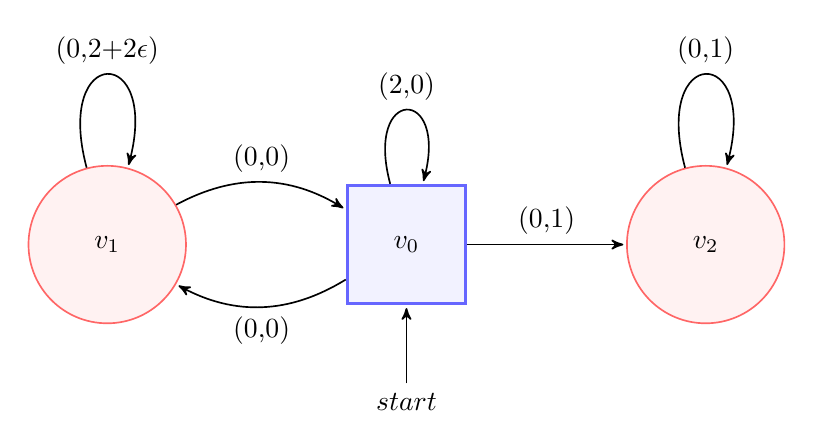
\begin{tikzpicture}[->,>=stealth',shorten >=1pt,auto,node distance=3.8cm,
                        semithick, squarednode/.style={rectangle, draw=blue!60, fill=blue!5, very thick, minimum size=15mm}]
      \tikzstyle{every state}=[fill=white,draw=black,text=black,minimum size=2cm]
    
      \node[squarednode]   (A)                    {$v_0$};
      \node[state, draw=red!60, fill=red!5]         (B) [left of=A] {$v_1$};
      \node[state, draw=red!60, fill=red!5]         (C) [right of=A] {$v_2$};
      \node[draw=none, fill=none, minimum size=0cm, node distance = 2cm]         (D) [below of=A] {$start$};
      \path (A) edge [bend left, below] node {(0,0)} (B)
                edge              node {(0,1)} (C)
                edge [loop above] node {(2,0)} (A)
            (B) edge [loop above] node {(0,2+2$\epsilon$)} (B)
                edge [bend left, above] node {(0,0)} (A)
            (C) edge [loop above] node {(0,1)} (C)
            (D) edge [left] node {} (A);
    \end{tikzpicture}
    \caption{Finite memory strategy of Player~$0$ may not achieve $\mathbf{ASV}^{\epsilon}(v_0)$}
    \label{fig:no_finite_strategy}
\end{figure}
\begin{proof}
Consider the example in Figure \ref{fig:no_finite_strategy}. We show that in this example $\mathbf{ASV}^{\epsilon}(v_0) = 1$, and that this $\mathbf{ASV}^{\epsilon}$ can only be achieved using an infinite memory strategy. Assume a strategy $\sigma_0$ for Player~0
such that the game is played in rounds.
In round $k$
% defined as: starting with $k=1$, repeat forever, 
\begin{itemize}[-]
    \item if Player~1 plays $v_0 \to v_0$ repeatedly at least $k$ times before playing $v_0 \to v_1$, then from $v_1$, play $v_1 \to v_1$ repeatedly $k$ times and then play $v_1 \to v_0$ and 
    % increment $k$ by 1, i.e., $k=k+1$; 
    move to round $k+1$;
    \item else, if Player~1 plays $v_0 \to v_0$ less than $k$ times before playing $v_0 \to v_1$, then from $v_1$ , play $v_1 \to v_0$.
\end{itemize}

The best response for Player~1 to strategy $\sigma_0$ would be to choose $k$ sequentially as $k = 1, 2, 3, \dotsc$, to get a play $\pi = ((v_0)^i(v_1)^i)_{i \in \mathbb{N}}$. We know that $\underline{\mathbf{MP}}_1(\pi) = 1+\epsilon$ and $\underline{\mathbf{MP}}_0(\pi) = 1$. Player~1 can sacrifice an amount that is less than $\epsilon$ to minimize mean-payoff of Player~0, and thus he would not like to play $v_0 \to v_2$. In particular, a strategy $\sigma_1$ of Player~1 that prescribes playing the edge $v_0 \to v_2$ some time 
% which is defined as playing $v_0 \to v_2$,
yields a mean-payoff of 1 for Player~1 and hence we conclude that $\sigma_1 \notin \mathbf{BR}_1^{\epsilon}(\sigma_0)$. Player~1 cannot play any other strategy without increasing the mean-payoff of Player~0 and/or decreasing his own payoff.
% Note that, it can be easily seen 
We can see that Player~1 does not have a finite memory best-response strategy. Thus, the $\mathbf{ASV}^{\epsilon}(\sigma_0)(v_0) = 1$.

% \mbcomment{We need to be more abstract about explaining the finite memory strategy}
We claim that $\mathbf{ASV}^{\epsilon}(\sigma_0)(v_0) = \mathbf{ASV}^{\epsilon}(v_0)$. For every strategy $\sigma_1$ of Player~1 such that $\sigma_1 \in \mathbf{BR}_1^{\epsilon}(\sigma_0)$, we note that the higher the payoff Player~1 has, the lower is the payoff for Player~0. For every other strategy, $\sigma_0'$, of Player~0, if best-response of Player~1 to $\sigma_0'$ gives a mean-payoff less than $1+\epsilon$, then Player~1 will switch to $v_2$, thus giving Player~0 a payoff of 0. If best-response of Player~1 to $\sigma_0'$ gives a mean-payoff greater than $1+\epsilon$, then Player~0 will have a lower $\mathbf{ASV}^{\epsilon}(\sigma_0')$.

Consider a finite memory strategy of Player~0. If Player~1 has an infinite memory response (that cannot be encoded by finite memory), it can only lead to looping over $v_0$ more and more, this gives him a payoff
which is eventually 0.

Now consider a finite memory response of Player~1 to the finite memory strategy of Player~0. Note that the resultant outcome is a regular path. Note that Player~0 would choose a finite memory strategy such that the
best response of Player~1 (which is achievable) gives him a value of at least $1 + \epsilon$. Also since both players have finite memory strategies, the resultant outcome is a regular path over vertices $v_0$ and $v_1$. In
every such regular path, the effect of the edge from $v_0$ to $v_1$ and the
edge from $v_1$ to $v_0$ is non-negligible, and hence if the Player~1 is at
least $1 + \epsilon$, the payoff of Player~0 will be less than 1. Thus no
finite memory strategy can achieve an $\mathbf{ASV}^{\epsilon}$ that is equal to 1. 
% Towards achieving $\mathbf{ASV}^{\epsilon}$, we can define an ideal finite memory strategy $\sigma_0^{FM}$ of Player~0 which would be of the form: repeat forever, if Player~1 plays $v_0 \to v_0$ repeatedly at least $l$ times before playing $v_0 \to v_1$, then Player~0 plays $v_1 \to v_1$ repeatedly $k$ times before playing $v_1 \to v_0$, where $l, k$ are some constants in $\mathbb{N}$. The best response of Player~1 to this strategy would be to play: repeat forever, play $v_0 \to v_0$ exactly $l$ times before playing $v_0 \to v_1$. Note that the mean-payoff of the best response is $\frac{(2+2\epsilon)\cdot k}{k + l + 2}$ and it must be greater than $1 + \epsilon$ to ensure Player~1 does not switch to playing $v_0 \to v_2$. Thus we get that $k \geqslant l + 2$. Player~0 benefits the most if she chooses $k = l+2$. Thus, we get a slightly modified strategy $\sigma_0^{FM'}$ of Player~0: repeat forever, if Player~1 plays $v_0 \to v_0$ repeatedly at least $l$ times before playing $v_0 \to v_1$, then Player~0 plays $v_1 \to v_1$ repeatedly $l+2$ times before playing $v_1 \to v_0$, where $l$ is  some constant in $\mathbb{N}$. Player~1's best response here is to play: repeat forever, play $v_0 \to v_0$ exactly $l$ times before playing $v_0 \to v_1$. Note that every other $\epsilon$-best response of Player~1 increases the payoff of Player~0. Thus, we get $\mathbf{ASV}^{\epsilon}(\sigma_0^{FM'}) = \frac{l}{l+2}$. By increasing $l \to \infty$, we can get $\mathbf{ASV}^{\epsilon}(\sigma_0^{FM'})$ very close to 1, but reaching 1 without infinite memory would not be possible. Thus, we see that the $\mathbf{ASV}^{\epsilon}$ can be reached only via an infinite memory strategy.
\end{proof}

The following example shows the existence of mean-payoff games in which Player $0$ can achieve the adversarial value with finite memory (but not memoryless) strategies.

\begin{theorem}
\label{ThmExNeedFinMem}
There exists a mean-payoff game $\mathcal{G}$ with vertex $v$ such that a finite memory of Player $0$ suffices to achieve $\mathbf{ASV}^{\epsilon}(v)$.
\end{theorem}
\begin{figure}
    \centering
    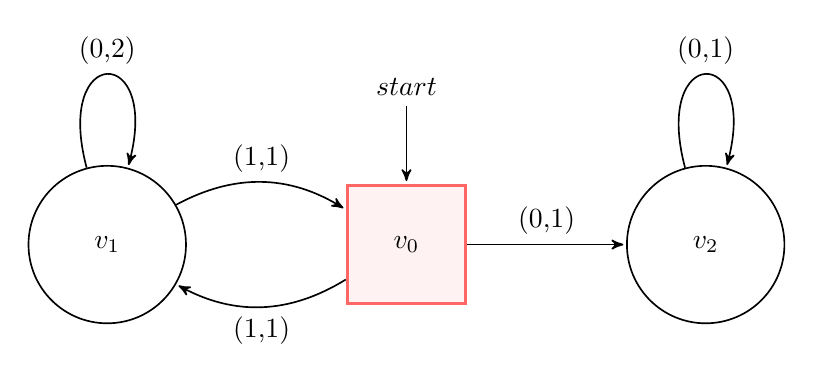
\begin{tikzpicture}[->,>=stealth',shorten >=1pt,auto,node distance=3.8cm,
                        semithick, squarednode/.style={rectangle, draw=red!60, fill=red!5, very thick, minimum size=15mm}]
      \tikzstyle{every state}=[fill=white,draw=black,text=black,minimum size=2cm]
    
      \node[squarednode]   (A)                    {$v_0$};
      \node[state]         (B) [left of=A] {$v_1$};
      \node[state]         (C) [right of=A] {$v_2$};
      \node[draw=none, fill=none, minimum size=0cm, node distance = 2cm]         (D) [above of=A] {$start$};
      \path (A) edge [bend left, below] node {(1,1)} (B)
                edge              node {(0,1)} (C)
            (B) edge [loop above] node {(0,2)} (B)
                edge [bend left, above] node {(1,1)} (A)
            (C) edge [loop above] node {(0,1)} (C)
            (D) edge [left] node {} (A);
    \end{tikzpicture}
    \caption{An example in which a finite memory strategy for Player $0$ suffices to achieve $\mathbf{ASV}^{\epsilon}(v_0)$.}
    \label{fig:finite_strategy_response}
\end{figure}
\begin{proof}
Consider the example in Figure \ref{fig:finite_strategy_response}. We show that $\mathbf{ASV}^{\epsilon}(v_0) = 1 - \epsilon$. Assume a strategy $\sigma_0^{k}$ for Player 0 defined as: repeat forever, from $v_1$ play one time $v_1 \to v_1$ and then repeat playing $v_1 \to v_0$ for $k$ times, with $k$ chosen such that mean-payoff for Player 0 is equal to $1 - \epsilon$. Such a $k$ always exists. The $\epsilon$-best response of Player 1 to $\sigma_0^{k}$ is to always play $v_0 \to v_1$, as by playing this edge forever, Player 1 gets a mean-payoff equal to $1+\epsilon$, where as if Player 1 plays $v_0 \to v_2$, then Player 1 is receives a payoff of $1$. Since $1 \ngtr (1 + \epsilon) - \epsilon$, the strategy $v_0 \to v_2$ does not fall under the $\epsilon$-best-response for Player 1, thus forcing Player 1 to play $v_0 \to v_1$. Thus $\mathbf{ASV}^{\epsilon}(v_0)$ is achieved with a finite memory of size $k$ for Player 0. Note that this size $k$ is a function of $\epsilon$.
\end{proof}

Further, we can also show that for a given strategy $\sigma_0$ of Player $0$, and for a given $\epsilon > 0$, there may not exist a finite memory strategy of Player $1$ that is an $\epsilon$-optimal response to $\sigma_0$.

\begin{theorem}
\label{ThmP1NeedInfMem}
There exists a mean-payoff game $\mathcal{G}$ such that for some Player $0$ strategy $\sigma_0$, for every strategy $\sigma_1$ of Player $1$, where $\sigma_1 \in \mathbf{BR}_1^{\epsilon}(\sigma_0)$, Player 1 needs infinite memory to play $\sigma_1$.
\end{theorem}
\begin{figure}
    \centering
    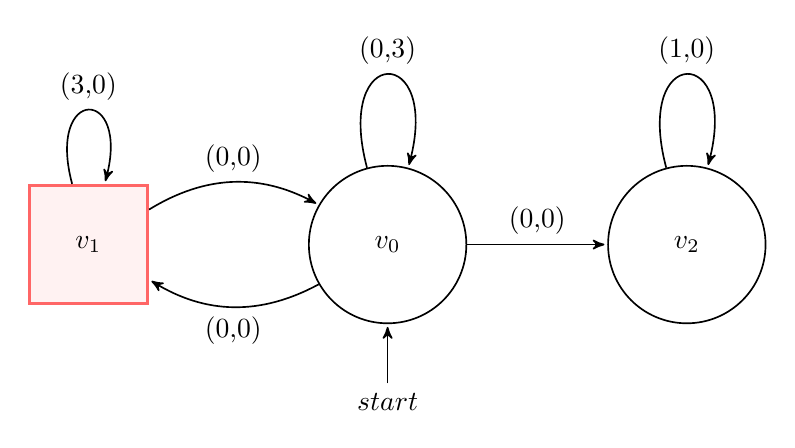
\begin{tikzpicture}[->,>=stealth',shorten >=1pt,auto,node distance=3.8cm,
                        semithick, squarednode/.style={rectangle, draw=red!60, fill=red!5, very thick, minimum size=15mm}]
      \tikzstyle{every state}=[fill=white,draw=black,text=black,minimum size=2cm]
    
      \node[state]   (A)                    {$v_0$};
      \node[squarednode]         (B) [left of=A] {$v_1$};
      \node[state]         (C) [right of=A] {$v_2$};
      \node[draw=none, fill=none, minimum size=0cm, node distance = 2cm]         (D) [below of=A] {$start$};
      \path (A) edge [bend left, below] node {(0,0)} (B)
                edge              node {(0,0)} (C)
                edge [loop above] node {(0,3)} (A)
            (B) edge [loop above] node {(3,0)} (B)
                edge [bend left, above] node {(0,0)} (A)
            (C) edge [loop above] node {(1,0)} (C)
            (D) edge [left] node {} (A);
    \end{tikzpicture}
    \caption{No $\epsilon$-optimal finite memory response of Player $1$ to a strategy $\sigma_0$ of Player $0$}
    \label{fig:no_optimal_response}
\end{figure}
\begin{proof}
Consider the example in Figure \ref{fig:no_optimal_response}.
Consider the following strategy $\sigma_0$ of Player $0$.
Player $0$ loops over $v_0$ $i$ times, and then sends the token to $v_1$.
Player $1$ loops over $v_1$ $k$ times, and then sends the token to $v_0$.
If $k \geqslant i$, then Player $0$ increases $i$ by $1$, and repeats the above, otherwise sends the token to $v_2$.
Clearly for all $\epsilon \leqslant 1.5$, no finite memory strategy only is an $\epsilon$ best response to $\sigma_0$.
\end{proof}

\section{Decision Problems for $\mathbf{ASV}^{\epsilon}$}
  In this section, we study the threshold problem of determining if $\mathbf{ASV}^{\epsilon}(v) > c$  for a given game $\mathcal{G}$ where $v$ is a vertex in $\mathcal{G}$ and $c$ is some rational constant.

We start by showing that if $\mathbf{ASV}^{\epsilon}(v) > c$, then there exists a strategy $\sigma_0$ for Player~0 that enforces $\mathbf{ASV}^{\epsilon}(\sigma_0)(v) > c$.

\begin{lemma}
\label{lem:witness_strategy}
For all mean-payoff games $\mathcal{G}$, for all vertices $v \in V$, for a fixed $\epsilon > 0$, we have that $\mathsf{ASV}^{\epsilon}(v) > c$ iff there exists a strategy $\sigma_0 \in \Sigma_0$ such that $\mathsf{ASV}^{\epsilon}(\sigma_0)(v) > c$.
\end{lemma}
\begin{proof}
% By definition of $\mathsf{ASV}^{\epsilon}(\sigma_0)(v) > c$, we have to show that:
% \begin{equation*}
%     \mathsf{ASV}^{\epsilon}(v) > c \iff \exists \sigma_0: \mathbf{BR}^{\epsilon}_1(\sigma_0) \neq \varnothing \land \forall \sigma_1 \in \mathbf{BR}^{\epsilon}_1(\sigma_0): \underline{\mathbf{MP}}_0(\mathbf{Out}_v(\sigma_0,\sigma_1)) > c
% \end{equation*}

\noindent The right to left direction of the proof is trivial as $\sigma_0$ can play the role of witness for $\mathsf{ASV}^{\epsilon}(v) > c$, i.e., if there exists a strategy $\sigma_0$ of Player $0$ such that $\mathsf{ASV}^{\epsilon}(\sigma_0)(v) > c$, then $\mathsf{ASV}^{\epsilon}(v) > c$.
% \\
% \noindent 

For the left to right direction of the proof, let $\mathsf{ASV}^{\epsilon}(v) = c'$. By definition of $\mathsf{ASV}^{\epsilon}( v)$, we have:
\begin{equation*}
    c' = \sup\limits_{\sigma_0 \in \Sigma_0}\mathsf{ASV}^{\epsilon}(\sigma_0)(v) 
\end{equation*}

\noindent By definition of $\sup$, for all $\delta > 0$, we have that:
\begin{equation*}
    \exists \sigma_0^{\delta}: \mathsf{ASV}^{\epsilon}(\sigma_0^{\delta})(v) \geqslant c' - \delta
\end{equation*}

\noindent Let us consider a $\delta > 0$ such that $c' - \delta > c$. Such a $\delta$ exists as $c' > c$. Then we obtain:
\begin{equation*}
    \exists \sigma_0: \mathsf{ASV}^{\epsilon}(\sigma_0)(v) \geqslant c' - \delta > c
\end{equation*}
\end{proof}

\noindent\textbf{Witnesses for $\mathbf{ASV}^{\epsilon}_{\mathsf{FM}}$} For a mean-payoff game $\mathcal{G}$ and an $\epsilon > 0$, we associate with each vertex $v$ in $\mathcal{G}$, the following set of pairs of real numbers:
\begin{equation*}
\Lambda^{\epsilon}(v) = \{(c,d) \in \mathbb{R}^2 \mid v \models \ll 1 \gg \underline{\mathbf{MP}}_0(\pi) \leqslant c \land \underline{\mathbf{MP}}_1(\pi) > d-\epsilon \}
\end{equation*}
We say that a vertex $v$ is $(c,d)^{\epsilon}$-bad if $(c,d) \in \Lambda^{\epsilon}(v)$. Let $c' \in \mathbb{R}$. A play $\pi$ in G is called a $(c',d)^{\epsilon}$-witness of $\mathbf{ASV}^{\epsilon}(v) > c$ if it starts from $v$, and $(\underline{\mathbf{MP}}_0(\pi), \underline{\mathbf{MP}}_1(\pi)) = (c', d)$ where $c' > c$, and $\pi$ does not contain any $(c,d)^{\epsilon}$-bad vertex. A play $\pi$ is called an $\epsilon$-witness of $\mathbf{ASV}^{\epsilon}(v) > c$ if it is a $(c',d)^{\epsilon}$-witness of $\mathbf{ASV}^{\epsilon}(v) > c$ for some $c',d$. 
The following theorem justifies the name witness.

\sgcomment{We should state the difficulty in our case compared to \cite{FGR20}.}

\begin{theorem}
\label{ThmWitnessASVInfMem}
For a given mean-payoff game $\mathcal{G}$ with a set $V$ of vertices, and for a vertex $v \in V$, we have that $\mathbf{ASV}^{\epsilon}(v) > c$ if and only if there exists a 
$(c',d)^{\epsilon}$-witness of $\mathbf{ASV}^{\epsilon}(v) > c$.
\end{theorem}
\begin{proof}
First we prove the right to left direction, i.e., we are given a play $\pi$ in $\mathcal{G}$ that starts from $v$   and the path $\pi$ is such that $(\underline{\mathbf{MP}}_0(\pi), \underline{\mathbf{MP}}_1(\pi)) = (c', d)$ for $c' > c$ and does not cross a $(c,d)^{\epsilon}$-bad vertex. We need to prove that $\mathbf{ASV}^{\epsilon}(v) > c$.
\\
\\
We do this by defining a strategy $\sigma_0$ for Player~0, such that $\mathbf{ASV}^{\epsilon}(\sigma_0)(v) > c$:
\begin{enumerate}
    \item $\forall h \leqslant \pi$, and $last(h)$ is a Player~0 vertex, the strategy $\sigma_0$ is such that $\sigma_0(h)$ follows $\pi$.
    \item $\forall h \nleqslant \pi$, where there has been a deviation from $\pi$ by Player~1, we assume Player~0 switches to a strategy that we call \textit{punishing}. This strategy is defined as follows: In the subgame after history $h'$ where ${\sf last}(h')$ is the first vertex from which Player~1 deviate from $\pi$, we know that Player~0 has a strategy to enforce the objective: $\underline{\mathbf{MP}}_0(\pi) > c$ $\lor$ $ \underline{\mathbf{MP}}_1(\pi) \leqslant d-\epsilon$. This is true because $\pi$ does not cross any $(c,d)^{\epsilon}$-bad vertex and since $n$-dimensional mean-payoff games are determined.
\end{enumerate}

Let us now establish that the strategy $\sigma_0$ satisfies $\mathbf{ASV}^{\epsilon}(\sigma_0)(v) > c$. 
First note that, since $\underline{\mathbf{MP}}_1(\pi) = d$, we have that $\sup\limits_{\sigma_1 \in \mathbf{BR}_1^{\epsilon}(\sigma_0)} \underline{\mathbf{MP}}_1(\mathbf{Out}(\sigma_0, \sigma_1)) \geqslant d$. Now consider some strategy $\sigma_1' \in \mathbf{BR}_1^{\epsilon}(\sigma_0)$ and let $\pi' = \mathbf{Out}(\sigma_0, \sigma_1')$. Clearly, $\pi'$ is such that $\underline{\mathbf{MP}}_1(\pi') > \sup\limits_{\sigma_1 \in \mathbf{BR}_1^{\epsilon}(\sigma_0)} \underline{\mathbf{MP}}_1(\mathbf{Out}(\sigma_0, \sigma_1)) -\epsilon \geqslant d-\epsilon$. If $\pi' = \pi$, we know that $\underline{\mathbf{MP}}_0(\pi') > c$. If $\pi' \neq \pi$, then when $\pi'$ deviates from $\pi$ we know that Player~0 employs a punishing strategy, thus making sure that $\underline{\mathbf{MP}}_0(\pi') > c$ $\lor$ $ \underline{\mathbf{MP}}_1(\pi') \leqslant d-\epsilon$. Since $\sigma_1' \in \mathbf{BR}_1^{\epsilon}(\sigma_0)$, it must be true that $\underline{\mathbf{MP}}_0(\pi') > c$. Thus, $\forall \sigma_1' \in \mathbf{BR}_1^{\epsilon}(\sigma_0)$, we have $\underline{\mathbf{MP}}_0(\mathbf{Out}(\sigma_0, \sigma_1')) > c$. Therefore, $\mathbf{ASV}^{\epsilon}(\sigma_0)(v) > c$, which implies $\mathbf{ASV}^{\epsilon}(v) > c$.

Now we consider the left to right direction of the proof, i.e., we are given that $\mathbf{ASV}^{\epsilon}(v) > c$. 
Hence by \textbf{\cref{lem:witness_strategy}}, there exists a strategy $\sigma_0$ for Player $0$ such that $\mathbf{ASV}^{\epsilon}(\sigma_0)(v) > c$. Thus, for some $\delta > 0$, we have:
\begin{equation*}
    \inf\limits_{\sigma_1 \in \mathbf{BR}_1^{\epsilon}(\sigma_0)} \underline{\mathbf{MP}}_0(\mathbf{Out}(\sigma_0, \sigma_1)) = c' = c + \delta
\end{equation*}
Let $d = \sup\limits_{\sigma_1 \in \mathbf{BR}_1^{\epsilon}(\sigma_0)} \underline{\mathbf{MP}}_1(\mathbf{Out}(\sigma_0, \sigma_1))$. We first prove that for all $\sigma_1 \in \mathbf{BR}_1^{\epsilon}(\sigma_0)$, we have that $\mathbf{Out}_v(\sigma_0, \sigma_1)$ does not cross a $(c,d)^{\epsilon}$-bad vertex. For every $\sigma_1 \in \mathbf{BR}_1^{\epsilon}(\sigma_0)$, we let $\pi_{\sigma_1} = \mathbf{Out}_v(\sigma_0, \sigma_1)$. We note that $\underline{\mathbf{MP}}_1(\pi_{\sigma_1}) > d -\epsilon$ and $\underline{\mathbf{MP}}_0(\pi_{\sigma_1}) > c$. For every $\pi' \in \mathbf{Out}_v(\sigma_0)$, we know that if $\underline{\mathbf{MP}}_1(\pi') > d - \epsilon$, then there exists a strategy $\sigma_1' \in \mathbf{BR}_1^{\epsilon}(\sigma_0)$ such that $\pi' = \mathbf{Out}_v(\sigma_0, \sigma_1')$. This means that $\underline{\mathbf{MP}}_0(\pi') > c$. Thus we can see that every deviation from $\pi_{\sigma_1}$ either gives Player~1 a mean-payoff less than $d - \epsilon$ or Player~0 a mean-payoff greater than $c$. Therefore, we conclude that $\pi_{\sigma_1}$ does not cross any $(c,d)^{\epsilon}$-bad vertex. 

Now consider a sequence ($\sigma_i$)$_{i \in \mathbb{N}}$ of Player $1$ strategies such that $\sigma_i \in \mathbf{BR}_1^{\epsilon}(\sigma_0)$ for all $i \in \mathbb{N}$, and $\lim \limits_{i \to \infty} \underline{\mathbf{MP}}_1(\mathbf{Out}(\sigma_0, \sigma_i))=d$. Let $\pi_i = \mathbf{Out}(\sigma_0, \sigma_i)$.
Let $\inf(\pi_i)$ be the set of vertices that occur infinitely often in $\pi_i$, and let $V_{\pi_i}$ be the set of vertices appearing along the path $\pi_i$.
W.l.o.g., since there are finitely many SCCs, we can assume that let for all $i, j \in \mathbb{N}$, we have that $\inf(\pi_i) = \inf(\pi_j)$, that is, all the paths end up in the same SCC, say $S$, and also $V_{\pi_i} = V_{\pi_j}=V_{\pi}$ (say). 
Note that $S \subseteq V_{\pi}$.
For all vertices $v$ in the SCC $S$, we know that $v$ is not $(c'',d)^{\epsilon}$-bad for $c'\geqslant c''> c$.

Note that for every $\epsilon \ge \delta > 0$, there is a strategy $\sigma_1^\delta \in \mathbf{BR}_1^{\epsilon}(\sigma_0)$ of Player $1$, and a corresponding path $\pi' = \mathbf{Out}_v(\sigma_0, \sigma_1^\delta)$ such that $\underline{\mathbf{MP}}_1(\pi') > d-\delta$, and $\underline{\mathbf{MP}}_0(\pi') \geqslant c''$.
Also the set $V_{\pi'}$ of vertices appearing in $\pi'$ be such that $V_{\pi'} \subseteq V_\pi$, and $\inf(\pi') \subseteq S$.

Now since $F_{\mathsf{min}}(\mathbb{CH}(\mathbf{C}(S)))$ is a closed set, we have that $(c'',d) \in F_{\mathsf{min}}(\mathbb{CH}(\mathbf{C}(S)))$.
By \textbf{\cref{lemCHToPlay}}, there exists a play $\pi^*$ such that $(\underline{\mathbf{MP}}_0(\pi^*), \underline{\mathbf{MP}}_1(\pi^*)) = (c'',d)$.
Also $\inf(\pi^*) \subseteq S$, and $V_{\pi^*} \subseteq V_{\pi}$.
The proof follows since for all vertices $v \in V_\pi$, we have that $v$ is not $(c'',d)^{\epsilon}$-bad for $c'' > c$.
% $\inf(\pi^*) \subseteq S$, and $V_{\pi^*} \subseteq V_{\pi}$, and $(\underline{\mathbf{MP}}_0(\pi^*), \underline{\mathbf{MP}}_1(\pi^*)) = (c^*,d)$. We observe that $\pi^*$ does not cross a $(c,d)^{\epsilon}$-bad vertex since $V_{\pi^*} \subseteq V_{\pi}$, and thus is an $\epsilon$-witness to $\mathbf{ASV}^{\epsilon}(v) > c$.
\end{proof}

\begin{figure}
    \centering
    \begin{tikzpicture}
        \tkzDefPoint(0,0){O}
        \tkzDefPoint(8,0){P}
        \tkzDefPoint(8,5){Q}
        \tkzDefPoint(0,5){R}
        \tkzDefPoint(2.5,0){X}
        \tkzDefPoint(1.25,0){X'}
        \tkzDefPoint(8,3){Y}
        \tkzDefPoint(2.5,5){Z}
        \tkzDefPoint(0,3){W}
        \tkzDrawSegments(O,P P,Q Q,R R,O X,Z Y,W)
        \tkzDefPoint(5.5,0){A}
        \tkzDefPoint(2.5,3){B}
        \tkzDefPoint(1.25,3){B'}
        \tkzCalcLength(X,A)\tkzGetLength{radius}
        \tkzDrawArc[R with nodes, color=blue](X,\radius pt)(A,B)
        \tkzDrawArc[R with nodes, color=red](X',\radius pt)(A,B)
        \tkzDrawArc[R with nodes, color=red, style=dashed](X',\radius pt)(A,B')
        \tkzDrawPoints(B, B')
        \tkzLabelPoint[above](B'){$(< c', d)$}
        \tkzLabelPoint[above](B){$(c', d)$}
        \tkzLabelPoint[above](Z){$x = c'$}
        \tkzLabelPoint[right](Y){$y = d$}
    \end{tikzpicture}
    \caption{Plot of mean-payoffs when approaching the limit}
    \label{fig:plot_mp_limit}
\end{figure}

% Since $F_{\mathsf{min}}(\mathbb{CH}(\mathbf{C}(S)))$ is a closed set, we have that $(c^*, d) \in \mathbf{CH(\mathbb{C}(\emph{S}))}$ for some $c^* \in \mathbb{Q}$. We now show that $c^* \geqslant c' = c+\delta$ and at the limit when $i\to \infty$, we have that mean-payoff of Player~1 in $\pi_i$ approaches $d$ and mean-payoff of Player~0 in $\pi_i$ is greater than or equal to $c'$. We prove this by contradiction. 

To give some intuition about the left to right direction of the proof, we consider the plots in Figure \ref{fig:plot_mp_limit}. The $x$-coordinates represent Player~0's mean-payoff, the $y$-coordinates represent Player~1's mean-payoff. The blue line depicts the set of plays $\pi_i$ such that when mean-payoff of Player~1 approaches $d$, mean-payoff of Player~0 approaches $c^* = c'$. Assume for contradiction that $c^* < c'$, i.e., we consider a set of outcomes $\pi_i$, where $\pi_i=\mathbf{Out}(\sigma_0, \sigma_i)$ and $\sigma_i \in \mathbf{BR}_1^{\epsilon}(\sigma_0)$, such that when mean-payoff of Player~1 approaches $d$, mean-payoff of Player~0 approaches $c^* < c'$. The red line on the graph plots such a set of $\pi_i$s. We note that, in the second case, that there exists outcomes ,$\pi_i$, as represented on graph by the red dashes, where $\underline{\mathbf{MP}}_0(\pi_i) < c'$ and $\underline{\mathbf{MP}}_1(\pi_i) < d$. This is a contradiction as the $\inf\limits_{\sigma_1 \in \mathbf{BR}_1^{\epsilon}(\sigma_0)} \underline{\mathbf{MP}}_0(\mathbf{Out}(\sigma_0, \sigma_1)) = c' = c + \delta$. 

% Thus, we conclude $c^* \geqslant c'$. 

Now, we establish \textbf{NP}-membership for the threshold problem of determining if $\mathbf{ASV}^{\epsilon}(v) > c$. Towards this, we first prove the following lemma.

\begin{lemma}
\label{LemPlaysAsWitnessForASV}
Given a mean-payoff game $\mathcal{G}$, a vertex $v$, an $\epsilon > 0$ and $c \in \mathbb{Q}$, we have that  $\mathbf{ASV}^{\epsilon}(v) > c$ if and only if there exist three acyclic plays $\pi_1, \pi_2, \pi_3$, and two simple cycles $l_1 , l_2$ such that:
\begin{enumerate}
    \item \textit{first}($\pi_1$) $ = v$, \textit{first}($\pi_2$) = \textit{last}($\pi_1$), \textit{first}($\pi_3$) = \textit{last}($\pi_2$), \textit{first}($\pi_2$) = \textit{last}($\pi_3$), and \textit{first}($\pi_2$) = \textit{first}($l_1$), and \textit{first}($\pi_3$) = \textit{first}($l_2$).
    \item there exists $\alpha, \beta \in \mathbb{Q}^{+}$, where $\alpha + \beta = 1$, such that:
    \begin{enumerate}
        \item $\alpha \cdot w_0(l_1) + \beta \cdot w_0(l_2) = c' > c$
        \item $\alpha \cdot w_1(l_1) + \beta \cdot w_1(l_2) = d$
    \end{enumerate}
    \item there is no $(c,d)^{\epsilon}$-bad vertex $v'$ along $\pi_1, \pi_2, \pi_3, l_1$ and $l_2$.
\end{enumerate}
\end{lemma}
\begin{proof}
This proof is similar to the proof of \textbf{Lemma 10} in \cite{FGR20}. 
For the right to left direction of the proof, where we are given finite acyclic plays $\pi_1, \pi_2, \pi_3$, simple cycles $l_1$ and $l_2$ and constants $\alpha, \beta$, we consider the witness $\pi = \pi_1\rho_1\rho_2\rho_3\dots$ where, for all $i \in \mathbb{N}$, we let $\rho_i = l_1^{[\alpha i]}.\pi_2.l_2^{[\beta i]}.\pi_3$. 
We know that $\underline{\mathbf{MP}}_1(\pi) = \alpha \cdot w_1(l_1) + \beta \cdot w_1(l_2) = d$ and $\underline{\mathbf{MP}}_0(\pi) = \alpha \cdot w_0(l_1) + \beta \cdot w_0(l_2) > c$. For all vertices $v$ in $\pi_1, \pi_2, \pi_3, l_1$ and $l_2$, it is given that $v$ is not $(c,d)^\epsilon$-bad. 
Therefore, $\pi$ is a suitable $\epsilon$-witness thus proving from \textbf{\cref{ThmWitnessASVInfMem}} that $\mathbf{ASV}^{\epsilon}(v) > c$.

We can optimize the $\epsilon$-witness $\pi$ by constructing an $\epsilon$-regular-witness $\pi'$ for $\mathbf{ASV}^{\epsilon}(v) > c$ where $\pi' = \pi_1.(l_1^{[\alpha']k}.\pi_2.l_2^{[\beta']k}.\pi_3)^{\omega}$ and $\alpha', \beta'$ are constants in $\mathbb{Q}$ and $k$ is some large constant in $\mathbb{N}$. We construct $\pi'$ by modifying $\pi$ as follows:
\begin{caseof}
    \case{$w_0(l_1) > w_0(l_2)$ and $w_1(l_1) < w_1(l_2)$}
    Here, one simple cycle, $l_1$, increases Player~0's mean-payoff while the other simple cycle, $l_2$, increases Player~1's mean-payoff. We can build a witness $\pi' = \pi_1.(l_1^{[\alpha]k}.\pi_2.l_2^{[\beta+\tau]k}.\pi_3)^{\omega}$ for some very large $k \in \mathbb{N}$ and for some very small $\tau > 0$ such that $\underline{\mathbf{MP}}_0(\pi') > c$ and $\underline{\mathbf{MP}}_1(\pi') = d$.\footnote{For more details, we refer the reader to the Appendix.}
    \case{$w_0(l_1) < w_0(l_2)$ and $w_1(l_1) > w_1(l_2)$}
    This is analogous to \textbf{case 1}, and proceeds as mentioned above.
    \case{$w_0(l_1) < w_0(l_2)$ and $w_1(l_1) < w_1(l_2)$}
    One cycle, $l_2$, increases both Player~0 and Player~1's mean-payoffs, while the other, $l_1$, decreases it. In this case, we can just omit one of the cycles - whichever cycle gives a larger mean-payoff, to get a finite memory strategy. Thus, $\pi' = \pi_1.l_2^{\omega}$ and we get $\underline{\mathbf{MP}}_0(\pi') > c$ , $\underline{\mathbf{MP}}_1(\pi') \geqslant d$.
    \case{$w_0(l_1) > w_0(l_2)$ and $w_1(l_1) > w_1(l_2)$}
    This is analogous to \textbf{case 3} and proceeds as mentioned above.
\end{caseof}
In each of these cases, we can show that $\pi'$ is a witness for $\mathbf{ASV}^{\epsilon}(v) > c$: $\underline{\mathbf{MP}}_0(\pi') > c$ and $\underline{\mathbf{MP}}_1(\pi') \geqslant d$.
Since we know that $\pi$ does not cross a $(c,d)^{\epsilon}$-bad vertex, the modified play $\pi'$ does not either, as the vertices of the play $\pi'$ are a subset of the vertices of the play $\pi$. 

For the left to right direction of the proof, we are given $\mathbf{ASV}^{\epsilon}(v) > c$. We can construct a path $\pi$ from \textbf{\cref{ThmWitnessASVInfMem}} such that $\underline{\mathbf{MP}}_0(\pi) > c$ and $\underline{\mathbf{MP}}_1(\pi) = d$ and $\pi$ does not cross a $(c,d)^{\epsilon}$-bad vertex, i.e., for all vertices $v'$ appearing in $\pi$, we have that $v' \nvDash \ll 1 \gg \underline{\mathbf{MP}}_0(\pi) \leqslant c \land \underline{\mathbf{MP}}_1(\pi) > d-\epsilon$. Let $\inf(\pi) = S$ be the set of vertices appearing infinitely often in $\pi$. Note that $S$ forms an SCC. 
Following the proof in \textbf{Lemma 10} in \cite{FGR20} and applying the Carathéodory baricenter theorem, we can find two simple cycles $l_1, l_2$ in $S$ and acyclic finite plays $\pi_1, \pi_2 $ and $\pi_3$ from $\pi$ and two positive rational constants $\alpha, \beta \in \mathbb{Q^+}$, such that, \textit{first}($\pi_1$) $ = v$, \textit{first}($\pi_2$) = \textit{last}($\pi_1$), \textit{first}($\pi_3$) = \textit{last}($\pi_2$), \textit{first}($\pi_2$) = \textit{last}($\pi_3$), and \textit{first}($\pi_2$) = \textit{first}($l_1$), and \textit{first}($\pi_3$) = \textit{first}($l_2$), and $\alpha + \beta = 1$, $\alpha \cdot w_0(l_1) + \beta \cdot w_0(l_2) > c$ and $\alpha \cdot w_1(l_1) + \beta \cdot w_1(l_2) = d' \geqslant d$. We note that for all vertices $v$ in $\pi_1, \pi_2, \pi_3, l_1$ and $l_2$, we have that $v$ is not $(c,d)^{\epsilon}$-bad and thus will not be $(c,d')^{\epsilon}$-bad.
\end{proof}

Now, we state the following theorem that establishes the $\mathbf{NP}$-membership of $\mathbf{ASV}^{\epsilon}(v) > c$.
\begin{theorem}
\label{ThmNpForASV}
Given a mean-payoff game $\mathcal{G}$, a vertex $v \in V$, a rational value $c \in \mathbb{Q}$ and $\epsilon > 0$, it can be decided in non-deterministic polynomial time if $\mathbf{ASV}^{\epsilon}(v) > c$.
\end{theorem}

\noindent The rest of this section is devoted towards proving \textbf{\cref{ThmNpForASV}}. We start by stating a property of multi-dimensional mean-payoff games proved in \cite{VCDHRR15} that we rephrase here for a 2-dimensional game:

\begin{lemma}
    \label{LemWeightPlayGrtThanC}
    In a mean-payoff game $\mathcal{G}$, if Player 0 wins $\underline{\mathbf{MP}}_0 < c \lor \underline{\mathbf{MP}}_1 < d$ from a vertex $v$ then he has a memoryless winning strategy $\sigma_0$ to do so, and there exist three constants $m_\mathcal{G}, c_\mathcal{G}, d_\mathcal{G} \in \mathbb{R}$ such that: $c_\mathcal{G} < c, d_\mathcal{G} < d$, and for all finite plays $\pi^f \in \mathbf{Out}_v(\sigma_0)$, i.e. starting in $v$ and compatible with $\sigma_0$, we have that:
    \begin{equation*}
        w_0(\pi^f) \leqslant m_\mathcal{G} + c_\mathcal{G} \times |\pi^f|
    \end{equation*}
    or
    \begin{equation*}
        w_1(\pi^f) \leqslant m_\mathcal{G} + d_\mathcal{G} \times |\pi^f|
    \end{equation*}
\end{lemma}

\noindent Then we prove the following result:

\begin{lemma}
    \label{ConjGrtIsGrtEq}
    For every mean payoff game $\mathcal{G}$, for all vertices $v \in \mathcal{G}$, for all rational constants $c, d \in \mathbb{Q}$, we have that:
    \begin{equation*}
        v \models \ll 1 \gg \underline{\mathbf{MP}}_0 \geqslant c \land \underline{\mathbf{MP}}_1 > d
    \end{equation*}
    if and only if there exists a rational constant $d' \in \mathbb{Q}$, where $d' > d$ such that
    \begin{equation*}
        v \models \ll 1 \gg \underline{\mathbf{MP}}_0 \geqslant c \land \underline{\mathbf{MP}}_1 \geqslant d'
    \end{equation*}
\end{lemma}

\begin{proof}
    For the right to left direction of the proof, it is trivial to see that 
    % if $\underline{\mathbf{MP}}_1 > d'$ for some $d' > d$ then this implies $\underline{\mathbf{MP}}_1 \geqslant d$. Hence we get that 
    if $v \models \ll 1 \gg \underline{\mathbf{MP}}_0 \geqslant c \land \underline{\mathbf{MP}}_1 \geqslant d'$ for some $d' > d$, then we have that $v \models \ll 1 \gg \underline{\mathbf{MP}}_0 \geqslant c \land \underline{\mathbf{MP}}_1 > d$.

    For the left to right direction of the proof, we prove the contrapositive, i.e., we assume that $\forall d' > d$, we have $v \nvDash \ll 1 \gg \underline{\mathbf{MP}}_0 \geqslant c \land \underline{\mathbf{MP}}_1 \geqslant d'$. Now we prove that $v \nvDash \ll 1 \gg \underline{\mathbf{MP}}_0 \geqslant c \land \underline{\mathbf{MP}}_1 > d$.

    Since $\forall d'> d$, Player 1 loses $\underline{\mathbf{MP}}_0 \geqslant c \land \underline{\mathbf{MP}}_1 \geqslant d'$ from a given vertex $v$, due to determinacy of multi-dimensional mean-payoff games, Player 0 wins $\underline{\mathbf{MP}}_0 < c \lor \underline{\mathbf{MP}}_1 < d'$ from the same vertex $v$. By \textbf{\Cref{LemWeightPlayGrtThanC}}, we have that Player 0 has a memoryless strategy $\sigma_0$ to achieve the objective $\underline{\mathbf{MP}}_0 < c \lor \underline{\mathbf{MP}}_1 < d'$ from the vertex $v$. Note that in a finite game $\mathcal{G}$, Player 0 has only finitely many memoryless strategy. Therefore there must exist at least one strategy $\sigma_0^*$ that achieves the objective $v \models \ll 0 \gg \underline{\mathbf{MP}}_0 < c \lor \underline{\mathbf{MP}}_1 < d'$ for all $d' > d$. From \textbf{\Cref{LemWeightPlayGrtThanC}}, we also get three constants $m_\mathcal{G}, c_\mathcal{G}, d_\mathcal{G} \in \mathbb{R}$ such that for all $d' > d$, we have that $c_\mathcal{G} < c, d_\mathcal{G} < d'$ and for all finite plays $\pi^f \in \mathbf{Out}_v(\sigma_0^*)$, we have that
    \begin{equation*}
        w_0(\pi^f) \leqslant m_\mathcal{G} + c_\mathcal{G} \times |\pi^f|
    \end{equation*}
    or we have that
    \begin{equation*}
        w_1(\pi^f) \leqslant m_\mathcal{G} + d_\mathcal{G} \times |\pi^f|
    \end{equation*}

    Now, for every play $\pi \in \mathbf{Out}_v(\sigma_0^*)$, we know that $|\pi| \to \infty$. Thus, we get that:
    \begin{equation*}
        \underline{\mathbf{MP}}_0(\pi) = \frac{w_0(\pi)}{|\pi|} \leqslant \frac{m_\mathcal{G}}{|\pi|} + c_\mathcal{G}
    \end{equation*}
    or we have that
    \begin{equation*}
        \underline{\mathbf{MP}}_1(\pi) = \frac{w_1(\pi)}{|\pi|} \leqslant \frac{m_\mathcal{G}}{|\pi|} + d_\mathcal{G}
    \end{equation*}

    Since $|\pi| \to \infty$, the constant $\frac{m_\mathcal{G}}{|\pi|} \to 0$. Thus, we get $v \models \ll 0 \gg \underline{\mathbf{MP}}_0(\pi) \leqslant c_\mathcal{G} \lor \underline{\mathbf{MP}}_1(\pi) \leqslant d_\mathcal{G}$. Since we know that $c_\mathcal{G} < c, d_\mathcal{G} < d'$, we get that $v \models \ll 0 \gg \underline{\mathbf{MP}}_0(\pi) < c \lor \underline{\mathbf{MP}}_1(\pi) < d'$ for every $d' > d$. Thus, we get that  $v \models \ll 0 \gg \underline{\mathbf{MP}}_0(\pi) < c \lor \underline{\mathbf{MP}}_1(\pi) \leqslant d$. Therefore, by determinacy of multi-dimensional mean-payoff games, we have that $v \nvDash \ll 1 \gg \underline{\mathbf{MP}}_0 \geqslant c \land \underline{\mathbf{MP}}_1 > d$.
\end{proof}

\textbf{Modified Game:} We now construct a game $\mathcal{G'}$ from the given game $\mathcal{G}$ by multiplying the first dimension on each edge by -1. It is easy to see that, for all vertices $v$ in $\mathcal{G}$, we have that $v \nvDash \ll 1 \gg \underline{\mathbf{MP}}_0 \leqslant c \land \underline{\mathbf{MP}}_1 > d-\epsilon$ if and only if for the same vertex $v$ in the game $\mathcal{G'}$, we have $v \nvDash \ll 1 \gg \overline{\mathbf{MP}}_0 \geqslant -c \land \underline{\mathbf{MP}}_1 > d-\epsilon$ for some value $d \in \mathbb{Q}$. From \textbf{\cref{ConjGrtIsGrtEq}}, for the same vertex $v$, we have $v \nvDash \ll 1 \gg \overline{\mathbf{MP}}_0 \geqslant -c \land \underline{\mathbf{MP}}_1 \geqslant d'$, for some $d' \in \mathbb{R}$ and $d' > d - \epsilon$. \\ \noindent
We modify the game $\mathcal{G'}$ further by adding $c$ to the first dimension and subtracting $d'$ from the second dimension for all the edges in the game. Note that the edges and the vertices of both games $\mathcal{G}$ and $\mathcal{G'}$ are the same, the only difference between the two games being their edge weights.

\noindent Now, we state the following proposition:
\begin{proposition}
    \label{PropGamStrEqNewGamStr}
    For every vertex $v \in V$ in the game $\mathcal{G'}$, Player 0 (Player 1) can ensure that $v \nvDash \ll 1 \gg \overline{\mathbf{MP}}_0 \geqslant 0 \land \underline{\mathbf{MP}}_1 \geqslant 0$ ($v \models \ll 1 \gg \overline{\mathbf{MP}}_0 \geqslant 0 \land \underline{\mathbf{MP}}_1 \geqslant 0$) with a strategy $\sigma_0^{v}$ ($\sigma_1^{v}$) if and only if Player 0 (Player 1) can ensure that $v \nvDash \ll 1 \gg \underline{\mathbf{MP}}_0 \leqslant c \land \underline{\mathbf{MP}}_1 > d-\epsilon$ ($v \models \ll 1 \gg \underline{\mathbf{MP}}_0 \leqslant c \land \underline{\mathbf{MP}}_1 > d-\epsilon$) with the same strategy $\sigma_0^{v}$ ($\sigma_1^{v}$) from vertex $v$ in the game $\mathcal{G}$.
\end{proposition}

\noindent We also refer to the result for Multi-weighted two-player games with $\mathbf{MeanPayoffInfSup}$ objective \cite{VCDHRR15}.

\begin{theorem}
    \label{ThmMemlessStrForP2}
    \textbf{\emph{(Theorem 8 in \cite{VCDHRR15})}} For multi-dimensional two-player mean-payoff games with objective \\
    $\mathbf{MeanPayoffInfSup}(I,J) = \{\pi' \in \mathbf{Plays}(\mathcal{G}) \mid \forall i \in I : \underline{\mathbf{MP}}(\pi')_i \geqslant 0 \text{ and } \forall j \in J : \overline{\mathbf{MP}}(\pi')_j \geqslant 0\}$ for Player 1, the following assertions hold:
    \begin{enumerate}
        \item Winning strategies for Player 1 require infinite-memory in general, and memoryless winning strategies exist for Player 0. \footnote{Player 0 is called Player 2 in \cite{FGR20}}
        \item The problem of deciding whether a given vertex is winning for Player 1 is coNP-complete.
    \end{enumerate}
\end{theorem}

\textbf{Proof of \Cref{ThmNpForASV}:} According to the \textbf{\cref{LemPlaysAsWitnessForASV}}, we consider a non-deterministic Turing machine that establishes the membership to $\mathbf{NP}$ by guessing a reachable SCC $S$, a finite play $\pi_1$ to reach $S$ from $v$, two simple cycles $l_1, l_2$, along with two finite plays $\pi_2$ and $\pi_3$ that connects the two simple cycles, and parameters $\alpha, \beta \in \mathbb{Q}^{+}$. Note that the parameters $\alpha , \beta$ can be obtained by solving a linear program. Since linear programs are solvable in polynomial time, the values $\alpha$ and $\beta$ have polynomial size representation. Additionally, for each vertex $v'$ that appear along the plays $\pi_1, \pi_2$ and $\pi_3$, and on the simple cycles $l_1$ and $l_2$, the turing machine guesses a memoryless strategy $\sigma_0^{v'}$ for Player 0 that establishes $v' \nvDash \ll 1 \gg \underline{\textbf{MP}}_0 \leqslant c \land \underline{\textbf{MP}}_1 > d - \epsilon$ which means by determinacy of multi-dimensional mean-payoff games, that $v' \models \ll 0 \gg \underline{\textbf{MP}}_0 > c \lor \underline{\textbf{MP}}_1 \leqslant d - \epsilon$. We shall now establish the existence of these memoryless strategies. 
We start by construction of a modified mean-payoff game $\mathcal{G'}$ from the given game $\mathcal{G}$. Now, we get a modified objective for Player 0 in $\mathcal{G'}$, i.e., to get a memoryless strategy for Player 0 for all vertices $v \in \pi_1, \pi_2, \pi_3, l_1, l_2$ such that $v \nvDash \ll 1 \gg \overline{\mathbf{MP}}_0 \geqslant 0 \land \underline{\mathbf{MP}}_1 \geqslant 0$. The existence of a memoryless strategy for Player 0 which ensures her objective follows from \textbf{\Cref{ThmMemlessStrForP2}}

\noindent We formulate $\mathcal{G'}$ as a multi-weighted two-player game structure specified in \textbf{\cref{ThmMemlessStrForP2}} with $I = \{1\}$ and $J = \{0\}$. 
Thus, by \textbf{\cref{PropGamStrEqNewGamStr}}, if Player 0 has a strategy $\sigma_0^{v}$ to ensure $v \nvDash \ll 1 \gg \underline{\mathbf{MP}}_0 \leqslant c \land \underline{\mathbf{MP}}_1 > d-\epsilon$ from every vertex $v \in \pi_1, \pi_2, \pi_3, l_1, l_2$, the same strategy $\sigma_0^{v}$for every vertex $v$ appearing in $\pi_1, \pi_2, \pi_3, l_1, \text{ and } l_2$ in the game $\mathcal{G'}$ ensures $v \nvDash \ll 1 \gg \underline{\mathbf{MP}}_0 \geqslant 0 \land \underline{\mathbf{MP}}_1 \geqslant 0$. 
By \textbf{\cref{ThmMemlessStrForP2}}, since Player 0 wins the game $\mathcal{G}'$ from every vertex $v$ in $\pi_1, \pi_2, \pi_3, l_1, s \text{ and } l_2$, she has a memoryless strategy $\sigma_0^{v}$ to do so thus ensuring that $v \nvDash \ll 1 \gg \underline{\mathbf{MP}}_0 \leqslant c \land \underline{\mathbf{MP}}_1 > d - \epsilon$. 
There are polynomially many vertices, and the memoryless strategy $\sigma_0^{v}$ is checkable in $\mathsf{PTime}$ ensuring that the vertices along $\pi_1, \pi_2, \pi_3$ and $l_1, l_2$ are not $(c,d)^\epsilon$-bad, where $d = \alpha \cdot w_1(l_1) + \beta \cdot w_1(l_2)$.

\section{Computing the $\mathbf{ASV}^{\epsilon}$ value}
  Given a two-dimensional mean-payoff game $\mathcal{G}$, a vertex $v$ in $\mathcal{G}$, we now show how to compute $\mathbf{ASV}^{\epsilon}(v)$.
We first show a method to compute $\mathbf{ASV}^{\epsilon}(v)$ using the theory of reals with additions. This approach is very similar to the one followed in \cite{FGR20} with the difference that we use the formula $\Psi_v^{\epsilon}$ instead of $\Psi_v$ as has been described below.
This approach also gives us the necessary intuition to compute $\mathbf{ASV}^{\epsilon}(v)$, using a second method, by solving a set of linear programs (LP) leading to establishing an {\sf EXPTime} algorithm.
This second method is new to this work, and does not appear in \cite{FGR20}.
Moreover, \cite{FGR20} does not provide any complexity for the computation of $\mathbf{ASV}$. 
One can show that, with small modifications to our method involving solving linear programs, it is possible to compute $\mathbf{ASV}$ as well in {\sf EXPTime}.

In the previous \mychapter, we establish the existence of a notion of witness for the Adversarial Stackelberg value in non-zero sum two-player mean-payoff games. This notion of witness can be used to decide the threshold problem in $\mathbf{NP}$ time. We now show how to use this notion to effectively compute the $\mathbf{ASV}^{\epsilon}(v)$. To do this, we refer to the following lemma which has been established in \cite{FGR20}. 
In \cite{FGR20}, the set $\Lambda(v)$ has been defined as $\Lambda(v) = \{(c,d) \in \mathbb{R}^2 \mid v \models \ll 1 \gg \underline{\mathbf{MP}}_0 \leqslant c \land \underline{\mathbf{MP}}_1 \geqslant d \}$.

\begin{lemma}
\label{LemPsiToThrOfReal}
 \emph{[\textbf{Lemma 9} in \cite{FGR20}]}
 Given a mean-payoff game $\mathcal{G}$ and a vertex $v$ in $\mathcal{G}$, we can effectively construct a formula $\Psi_v(x, y)$ of $\langle \mathbb{R}, +, < \rangle$ with two free variables such that $(c,d) \in \Lambda(v)$ if and only if the formula $\Psi_v(x, y)[x/c, y/d]$ is true.
\end{lemma}

From the above lemma we can now compute an effective representation of the infinite set of pairs $\Lambda^{\epsilon}(v)$ for each vertex $v$ of the mean-payoff game in the following lemma:

\begin{lemma}
\label{LemPsiEpsToThrOfReal}
 Given a mean-payoff game $\mathcal{G}$ and a vertex $v$ in $\mathcal{G}$, we can effectively  construct a formula $\Psi_v^{\epsilon}(x, y)$ of $\langle \mathbb{R}, +, < \rangle$ with two free variables such that $(c,d) \in \Lambda^{\epsilon}(v)$ if and only if the formula $\Psi_v^{\epsilon}(x, y)[x/c, y/d]$ is true.
\end{lemma}
\begin{proof}
From the definition of $\Lambda(v)$ from \cite{FGR20}, we know that a pair of real values $(c,d) \in \Lambda(v)$ if $v \models \ll 1 \gg \underline{\mathbf{MP}}_0 \leqslant c \land \underline{\mathbf{MP}}_1 \geqslant d$.
We now recall from the definition of $\Lambda^{\epsilon}(v)$ that $(c,d) \in \Lambda^{\epsilon}(v)$ if $v \models \ll 1 \gg \underline{\mathbf{MP}}_0 \leqslant c \land \underline{\mathbf{MP}}_1 > d-\epsilon$.
From this, we can see that:
\begin{equation*}
    \Psi_v^{\epsilon}(x, y) \equiv \exists e > 0 \cdot \Psi_v(x, y - \epsilon + e)
\end{equation*}
\end{proof}

\textbf{Extended mean-payoff game} Similar to the approach of \cite{FGR20}, from the mean-payoff game $\mathcal{G} = (V, E, w_0, w_1)$,  we construct an extended mean-payoff game $\mathcal{G}^{\mathsf{ext}} = (V^{\mathsf{ext}}, E^{\mathsf{ext}}, w_0^{\mathsf{ext}}, w_1^{\mathsf{ext}})$, whose vertices and edges are defined as follows. The set of vertices is $V^{\mathsf{ext}} = V \times 2^V$. With a history $h$ in $\mathcal{G}$, we associate a vertex in $\mathcal{G}^{\mathsf{ext}}$ which is a pair $(v, P)$, where $v = last(h)$ and $P$ is the set of the vertices traversed along $h$. Accordingly the set of edges and the weight functions are defined as $E^{\mathsf{ext}} = \{((v,P),(v', P')) \mid (v,v') \in E \land P' = P \cup \{v'\}\}$ and $w_i^{\mathsf{ext}}((v,P),(v', P')) = w_i(v, v')$, for $i \in \{0,1\}$ Clearly, there exists a bijection between the plays $\pi$ in $\mathcal{G}$ and the plays $\pi^{\mathsf{ext}}$ in $\mathcal{G}^{\mathsf{ext}}$ which start in vertices of the form $(v, \{v\})$, i.e. $\pi^{\mathsf{ext}}$ is mapped to the play $\pi$ in $\mathcal{G}$ that is obtained by erasing the second dimension of its vertices.

We recall the following from \cite{FGR20}.
\begin{proposition}
\label{PropExtGamePlayConverges}
For all mean-payoff games $\mathcal{G}$, the following holds:

\begin{itemize}
    \item Let $\pi^{\mathsf{ext}}$ be an infinite play in the extended mean-payoff game and $\pi$ be its projection on the original mean-payoff game $\mathcal{G}$ (over the first component of each vertex), the following properties hold: \begin{itemize}
        \item For all $i < j$, if $\pi^{\mathsf{ext}}(i) = (v_i, P_i)$ and $\pi^{\mathsf{ext}}(j) = (v_j, P_j)$, then $P_i \subseteq P_j$
        \item $\underline{\mathbf{MP}}_i(\pi^{\mathsf{ext}}) = \underline{\mathbf{MP}}_i(\pi)$, for $i \in \{0,1\}$.
    \end{itemize}
    \item The unfolding of $\mathcal{G}$ from $v$ and the unfolding of $\mathcal{G}^{\mathsf{ext}}$ from $(v, \{v\})$ are isomorphic and so $\mathbf{ASV}^{\epsilon}(v) = \mathbf{ASV}^{\epsilon}(v, \{v\})$
\end{itemize}
\end{proposition}

By the first point of the above proposition and since the set of vertices of the mean-payoff game is finite, the second component of any play $\pi^{\mathsf{ext}}$ stabilises into a set of vertices of $\mathcal{G}$ which we denote by $V^{*}(\pi^{\mathsf{ext}})$. We now show how to characterize $\mathbf{ASV}^{\epsilon}(v)$ with the notion of witness introduced above and the decomposition of $\mathcal{G}^{\mathsf{ext}}$ into SCC. This is formalized in the following lemma:

\begin{lemma}
\label{LemASVMaxSCCExtGamePlay}
 For all mean-payoff games $\mathcal{G}$, for all vertices $v$ in $\mathcal{G}$, let $\mathsf{SCC}^{\mathsf{ext}}(v)$ be the set of strongly-connected components in $\mathcal{G}^{\mathsf{ext}}$ which are reachable from $(v, \{v\})$. Then we have
 \begin{equation*}
     \mathbf{ASV}^{\epsilon}(v) = \max \limits_{S \in \mathsf{SCC}^{\mathsf{ext}}(v)} \sup \{c \in \mathbb{R} \mid \exists \pi^{\mathsf{ext}}: \pi^{\mathsf{ext}} \textit{ is a witness for } \mathbf{ASV}^{\epsilon}(v, \{v\}) > c \textit{ and } V^{*}(\pi^{\mathsf{ext}}) = S \}
 \end{equation*}
\end{lemma}

\begin{proof}
First, we note the following sequence of inequalities:
\begin{equation*}
    \begin{split}
        \mathbf{ASV}^{\epsilon}(v) &= \sup \{ c \in \mathbb{R} \mid \mathbf{ASV}^{\epsilon}(v) \geqslant c \} \\
        &= \sup \{ c \in \mathbb{R} \mid \mathbf{ASV}^{\epsilon}(v) > c \} \\
        &= \sup \{ c \in \mathbb{R} \mid \exists \pi: \pi \textit{ is a witness for } \mathbf{ASV}^{\epsilon}(v) > c \} \\
        &= \sup \{ c \in \mathbb{R} \mid \exists \pi^{\mathsf{ext}}: \pi^{\mathsf{ext}} \textit{ is a witness for } \mathbf{ASV}^{\epsilon}(v, \{v\}) > c \} \\
        &= \max \limits_{S \in \mathsf{SCC}^{\mathsf{ext}}(v)} \sup \{ c \in \mathbb{R} \mid \exists \pi^{\mathsf{ext}}: \pi^{\mathsf{ext}} \textit{ is a witness for } \mathbf{ASV}^{\epsilon}(v, \{v\}) > c \textit{ and } V^{*}(\pi^{\mathsf{ext}}) = S \}
    \end{split}
\end{equation*}

The first two equalities are direct consequences of the definition of the supremum and that $\mathbf{ASV}^{\epsilon} \in \mathbb{R}$. The third is a consequence of \textbf{\cref{ThmWitnessASVInfMem}} that guarantees the existence of witnesses for strict inequalities. The fourth equality is a consequence of the second point in \textbf{\cref{PropExtGamePlayConverges}}. The last equality is the consequence of first point in \textbf{\cref{PropExtGamePlayConverges}}.
\end{proof}

By definition of $\mathcal{G}^{\mathsf{ext}}$, for every $\mathsf{SCC}$ $S$ of $\mathcal{G}^{\mathsf{ext}}$, there exists a set of vertices of $\mathcal{G}$ which we denote by $V^{*}(S)$ such that for every vertex of $S$ is of the form $(v, V^*(S))$. The set of bad thresholds for $S$ is then defined as $\Lambda^{\mathsf{ext}} = \bigcup_{v \in V^{*}(S)} \Lambda^{\epsilon}(v)$. Applying \textbf{\cref{LemPsiEpsToThrOfReal}}, we can now construct a formula $\Psi^{\epsilon}_{S}(x,y)$ which symbolically encodes the set $\Lambda^{\mathsf{ext}}$.

Now, we are equipped to prove that $\mathbf{ASV}^{\epsilon}(v)$ is effectively computable.
% This is expressed in the following theorem and established in its proof:

\begin{theorem}
\label{ThmComputeASV}
For all mean-payoff games $\mathcal{G}$, for all vertices $v$ in $\mathcal{G}$, the value $\mathbf{ASV}^{\epsilon}(v)$ can be effectively expressed by a formula $\rho_v$ in $\langle \mathbb{R}, +, < \rangle$ and computed from this formula.
\end{theorem}
\begin{proof}
\noindent To establish this theorem, we show how to build the formula $\rho_v(z)$ that is true iff $\mathbf{ASV}^{\epsilon}(v) = z$. We use \textbf{\cref{LemASVMaxSCCExtGamePlay}} to reduce this to the construction of a formula that expresses the existence of witness for $\mathbf{ASV}^{\epsilon}(v)$ from $(v, \{v\})$:
 \begin{equation*}
     \mathbf{ASV}^{\epsilon}(v) = \max \limits_{S \in \mathsf{SCC}^{\mathsf{ext}}(v)} \sup \{c \in \mathbb{R} \mid \exists \pi^{\mathsf{ext}}: \pi^{\mathsf{ext}} \textit{ is a witness for } \mathbf{ASV}^{\epsilon}(v, \{v\}) > c \textit{ and } V^{*}(\pi^{\mathsf{ext}}) = S \}
 \end{equation*}
 
\noindent As $\max \limits_{S \in \mathsf{SCC}^{\mathsf{ext}}(v)}$ is easily expressed in $\langle \mathbb{R}, +, < \rangle$, we concentrate on one $\mathsf{SCC}$ $S$ reachable from $(v, \{v\})$ and we show how to express
 \begin{equation*}
     \sup \{ c \in \mathbb{R} \mid \exists \pi^{\mathsf{ext}}: \pi^{\mathsf{ext}} \textit{ is a witness for } \mathbf{ASV}^{\epsilon}(v, \{v\}) > c \textit{ and } V^{*}(\pi^{\mathsf{ext}}) = S \}
 \end{equation*}

\noindent Such a value of $c$ can be encoded by the following formula:
% This is done by the following formula:
\begin{equation*}
    % \rho^S_{v_0}(z) \equiv \forall e > 0 \cdot \exists x,y \cdot x > z - e \land \Phi_S(x,y) \land \neg \Psi_S^{\epsilon}(z-e, y)
    \rho^S_{v_0}(c) \equiv \exists x,y \cdot x > c \land \Phi_S(x,y) \land \neg \Psi_S^{\epsilon}(c, y)
\end{equation*}

\noindent where $\Phi_S(x,y)$ is the symbolic encoding of $\Fmin{\CH{\CS}}$ as defined in \textbf{\cref{lemCHToPlay}}. This ensures that the values $(x,y)$ are the mean-payoff values realisable by some path in $S$. By \textbf{\cref{LemPsiEpsToThrOfReal}}, $\neg \Psi_S^{\epsilon}(c, y)$ expresses that the path does not cross a $(c, y)^{\epsilon}$-bad vertex. So the conjunction $\exists x,y \cdot x > c \land \Phi_S(x,y) \land \neg \Psi_S^{\epsilon}(c, y)$ establishes the existence of a witness with mean-payoff values $(x,y)$ for the threshold $c$, and hence satisfying this formula implies that $\mathbf{ASV}^{\epsilon}(v) > c$.
% The quantification over $e > 0$ expresses that $z$ is the sup over all the thresholds $z-e$ that have a witness.
Now we consider the formula
\begin{equation*}
    % \rho^S_{\max,v_0}(z) \equiv \forall x \cdot \rho^S_{v_0}(z) \land \rho^S_{v_0}(x) \implies z \geqslant x
    \rho^S_{\max,v_0}(z) \equiv \forall e > 0 \cdot \rho^S_{v_0}(z-e) \land \forall x \cdot \rho^S_{v_0}(x) \implies x < z
\end{equation*}
From this formula, we can compute the $\mathbf{ASV}^{\epsilon}$ by quantifier elimination in:
\begin{equation*}
    \max \limits_{S \in \mathsf{SCC}^{\mathsf{ext}}(v)} \exists z \cdot \rho^S_{\max,v_0}(z)
\end{equation*}
\noindent and obtain the unique value of $z$ that makes this formula true, and equals $\mathbf{ASV}^{\epsilon}(v)$.
\end{proof}

\begin{example}
\label{Ex:CompASVTOR}
\emph{Let us illustrate the computation of $\mathbf{ASV}^{\epsilon}$ with an example. Consider the mean-payoff game $\mathcal{G}$ depicted in \cref{fig:ach_example}.}
\begin{figure}
    \centering
    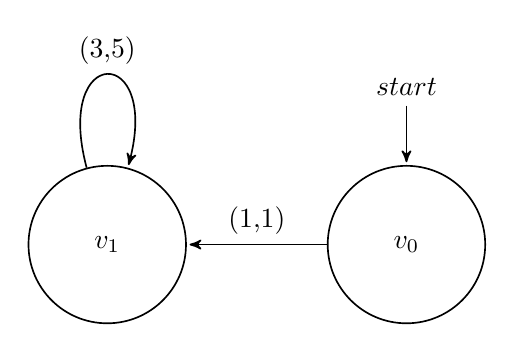
\begin{tikzpicture}[->,>=stealth',shorten >=1pt,auto,node distance=3.8cm, semithick]
      \tikzstyle{every state}=[fill=white,draw=black,text=black,minimum size=2cm]
    
      \node[state]         (A)             {$v_0$};
      \node[state]         (B) [left of=A] {$v_1$};
      \node[draw=none, fill=none, minimum size=0cm, node distance = 2cm]  (D) [above of=A] {$start$};
      \path (A) edge [right, above] node {(1,1)} (B)
            (B) edge [loop above] node {(3,5)} (B)
            (D) edge [left] node {} (A);
    \end{tikzpicture}
    \caption{Example to calculate $\mathbf{ASV}^{\epsilon}(v_0)$}
    \label{fig:ach_example}
\end{figure}
\emph{We note that in the mean-payoff game there exists exactly one $\mathsf{SCC}$ which is $S = \{v_1\}$ and it contains exactly one cycle $v_1 \to v_1$. Thus, $\Fmin{\CH{\CS}} = \{(3,5)\}$. 
% Note that if the $\mathsf{SCC}$ $S$ contained multiple cycles, the set $F_{\min}(\mathsf{CH}(\mathbb{C}(S)))$ can be expressed by a set of inequations. 
Thus, we get that $\Phi_S(x,y) \equiv x = 3 \land y = 5 $. 
Now $ \Lambda^{\epsilon}(v) = \{(c,d) \mid c \geqslant 3 \land d < 5 + \epsilon \}$,
and hence $\Psi_S^{\epsilon}(x, y) \equiv x \geqslant 3 \land y < 5 + \epsilon$.
% We note that the formula $\rho^S_{v_0}(z)$ holds for $z=3$, and by assigning $3$ to $x$, and $5$ to $y$.
We note that the formula $\rho^S_{v_0}(c)$ holds for values of $c$ less than $3$, and by assigning $3$ to $x$, and $5$ to $y$, and thus $\rho^S_{\max,v_0}(z)$ holds true for $z=3$.
% Since there is only path in the MDP, we have that $\rho^S_{\max,v_0}(z)$ also holds true for $z=3$.
It follows that $\mathbf{ASV}^{\epsilon}(v_0) = 3$ since we have a single SCC in the example.
% From \textbf{\cref{ThmComputeASV}}, we know that the formula to compute $\mathbf{ASV}^{\epsilon}$ is $\max \limits_{S \in \mathsf{SCC}^{\mathsf{ext}}(v)} \exists z \cdot \rho^S_{\max,v_0}(z)$. Since there is just one $\mathsf{SCC}$, the formula can be reduced to $\exists z \cdot \rho^S_{\max,v_0}(z)$, where $\rho^S_{\max,v_0}(z) \equiv \forall x \cdot \rho^S_{v_0}(z) \land \rho^S_{v_0}(x) \implies z \geqslant x$. Now, we know that $\rho^S_{v_0}(z) \equiv \forall e > 0 \cdot \exists x,y \cdot x > z - e \land \Phi_S(x,y) \land \neg \Psi_S^{\epsilon}(z-e, y)$. Substituting for $\Phi_S$ and $\Psi_S$, we get $\rho^S_{v_0}(z) \equiv \forall e > 0 \cdot \exists x,y \cdot x > (z - e) \land x = 3 \land y = 5 \land (z - e) \geqslant 3 \lor y \leqslant (5 + \epsilon)$. 
% Thus, the $\mathbf{ASV}^{\epsilon}(v_0) = 3$ which is unique value of $z$ that satisfies $\rho^S_{\max,v_0}(z)$.
}
\end{example}

\subsection{Computing $\mathbf{ASV}^{\epsilon}(v)$ by solving LP}
% \sgcomment{We are still working on this part.}
% We now develop an exponential time algorithm to compute $\mathbf{ASV}^{\epsilon}(v)$.
In this \mychapter, we provide another approach for computing $\mathbf{ASV}^{\epsilon}(v)$.
We use LP to solve the problem and obtain an $\mathsf{ExpTime}$ upper bound for the computation of $\mathbf{ASV}^{\epsilon}(v)$.
We do this by expressing the formula $\rho^S_{\max,v_0}$, for each $\mathsf{SCC}$ $S$, as a set of linear programs such that the maximum value over the set of solutions over all {\sf SCC}s corresponds to $\mathbf{ASV}^{\epsilon}$. 
We first illustrate our approach with the help of the following example.
% We now demonstrate the algorithm with an example:
\begin{example}
\label{Ex:CompASVLP}
\emph{Consider again
% Let us illustrate the polyhedron algorithm on 
the mean-payoff game $\mathcal{G}$ in \textbf{\cref{Ex:CompASVTOR}}.}
% depicted in \cref{fig:ach_example}.} 
\emph{We previously showed that the $\mathbf{ASV}^{\epsilon}(v_0)$ can be computed by quantifier elimination of a formula in the theory of reals with addition. Now, we compute $\mathbf{ASV}^{\epsilon}(v_0)$ by solving a set of linear programs for every $\mathsf{SCC}$ in $\mathcal{G}$.}
\emph{In this example, since there exists only one $\mathsf{SCC}$ $S = \{v_1\}$ in $\mathcal{G}$, we will have to solve only one linear program. 
% We start by expressing the set $F_{\min}(\mathsf{CH}(\mathbb{C}(S)))$ as a polyhedron, i.e.
In \cite{CDEHR10}, it has been shown that $\Fmin{\CH{\CS}}$ can be defined using a set of linear inequations.
Now recall from \cref{Ex:CompASVTOR} that $\Fmin{\CH{\CS}}=\{(3,5)\}$.
% \equiv \{x = 3, y = 5\}$. 
Note that $\Lambda^{\epsilon} = \{(c,y) \:|\: c \geqslant 3 \land y < 5 + \epsilon \}$.
% One crucial part to our approach is to compute $\Lambda^{'\epsilon}$ from $\Lambda^{\epsilon}$ by replacing the non-strict inequality in the first dimension with a strict inequality.
% Next, we compute the set of linear inequations which represents
% Thus we obtain $\Lambda'^{\epsilon} = \{(x,y) \:|\: x > 3 \land y < 5 + \epsilon \}$, and hence the system of inequations which represents $F_{\min}(\mathsf{CH}(\mathbb{C}(S))) \backslash \Lambda'^{\epsilon}(v)$ is given by $\{ x = 3 \land y = 5 \land (x \leqslant 3 \lor y \geqslant (5 + \epsilon)) \}$. 
% This is equivalent to having two linear programs: 
Thus the complement of $\Lambda^{\epsilon}(v_0)$, that is, $\bar{\Lambda}^{\epsilon}(v_0) = \mathbb{R} \times \mathbb{R} - \Lambda^{\epsilon}(v_0) = \{(c,y) \:|\: c < 3 \lor y \geqslant 5 + \epsilon \}$.
Now we emulate the formula $\rho_{v_0}^S(c)$ as $\exists x,y \models c<x \land x=3 \land y=5 \land (c \leqslant 3 \lor y \geqslant 5+\epsilon)$.
We maximise the value of $c$, which gives us the following two linear programs: \textit{maximise $c$ in $\exists x, y \models (c < x \land x = 3 \land y = 5 \land c \leqslant 3)$} and \textit{maximise x in $\exists x, y \models (c < x \land x = 3 \land y = 5 \land y \geqslant (5 + \epsilon))$} which yields the set of solutions: $\{3\}$. Thus, we conclude that $\mathbf{ASV}^{\epsilon}(v_0) = 3$.
Note that in an LP, the strict inequalities are replaced with non-strict inequalities.}
\end{example}

% Let us consider the mean-payoff game depicted in the example \cref{Ex:CompASVLP}. 
\begin{comment}
Note that when the mean-payoff $\mathcal{G}$ comprises of a single $\mathsf{SCC}$ $S$ which contains a single cycle and hence the set $F_{\min}(\mathsf{CH}(\mathbb{C}(S)))$ contains a single point $\{(x, y)\}$ where $x$ and $y$ represent the mean-payoff values of Player~0 and Player~1 respectively. 
Since Player~0 and Player~1 have a single strategy, the mean-payoff values $(x,y)$  are \textit{enforceable} by Player~1 and hence belong to $\Lambda^{\epsilon}(v)$. Thus, when we compute the set $F_{\min}(\mathsf{CH}(\mathbb{C}(S))) \backslash \Lambda^{\epsilon}(v)$, we get an empty set and therefore, the linear program yields no solution. We fix this problem, we convert the non-strict inequations in $\Lambda^{\epsilon}(v)$ to strict inequations, namely, $\Lambda'^{\epsilon}(v)$ and compute $F_{\min}(\mathsf{CH}(\mathbb{C}(S))) \backslash \Lambda'^{\epsilon}(v)$. 

Let us now consider the case when the mean-payoff game $\mathcal{G}$ comprises of a single $\mathsf{SCC}$ $S$ which contains two cycles with mean-payoff values $(x_1, y_1)$ and $(x_2, y_2)$ respectively. Note that the set $\mathsf{CH}(\mathbb{C}(S))$ comprises of points which lie on the line between $(x_1, y_1)$ and $(x_2, y_2)$ and therefore 
% the set $F_{\min}(\mathsf{CH}(\mathbb{C}(S)))$ represents a bounded area in the graph $\mathbb{R}^{2}$.
these points are also included in the set $F_{\min}(\mathsf{CH}(\mathbb{C}(S)))$.
On the other hand, note that all the mean-payoff values corresponding to these points may be enforceable by Player $1$, depending on who owns the vertices in $S$.
Assuming the slope of this line to be $m$, and its $y$-intercept to be $c$, for $\Lambda^{\epsilon}(v)$, the corresponding inequation is of the form $y \leqslant mx+c$, while in $\Lambda'^{\epsilon}(v)$, we use the strict inequation $y < mx+c$ instead.
Thus, when we compare the areas in the graph $\mathbb{R} \times \mathbb{R}$ generated by the sets $F_{\min}(\mathsf{CH}(\mathbb{C}(S))) \backslash \Lambda^{\epsilon}(v)$ and $F_{\min}(\mathsf{CH}(\mathbb{C}(S))) \backslash \Lambda'^{\epsilon}(v)$, we see that the only difference between the two sets lie in the boundary points, that is, the points in the line segment are excluded from the first set, while it is not the case for the second set.
% Since $\mathbf{ASV}^{\epsilon}(v)$ is computed as the $\sup$ of the set $\{ F_{\min}(\mathsf{CH}(\mathbb{C}(S))) \backslash \Lambda^{\epsilon}(v) \}$, replacing $\Lambda^{\epsilon}(v)$ with $\Lambda'^{\epsilon}(v)$ will still yield the same result. 
We can further extend this idea to all mean-payoff games which contain multiple $\mathsf{SCC}$s with each $\mathsf{SCC}$ containing multiple cycles.
\end{comment}

Now we state the main result of this \mychapter.
% This expressed in the following theorem.
\begin{theorem}
    \label{ExpTimeForComputeASV}
    For every mean-payoff game $\mathcal{G}$, for every vertex $v$ in $\mathcal{G}$, the value $\mathbf{ASV}^{\epsilon}(v)$ can be computed in $\mathsf{ExpTime}$.
\end{theorem}
\begin{proof}
The algorithm to compute $\mathbf{ASV}^{\epsilon}(v)$ is defined as follows:
\begin{enumerate}
    \item First we note that using 
    % \textbf{\cref{lemCHToPlay}} that we have that, 
    results from \cite{CDEHR10},
    for each $\mathsf{SCC}$ $S$ in the mean-payoff game $\mathcal{G}$, the set $\Fmin{\CH{\CS}}$ can be expressed as a set of exponentially many inequations.
    % \item From \textbf{\cref{LemPsiEpsToThrOfReal}}, we can compute a representation of $\Lambda^{\epsilon}(v)$ as a finite union of system of strict and non-strict inequations. Thus, we can represent the complement $(\mathbb{R}^2 - \Lambda^{\epsilon}(v))$ as a finite union of system of strict and non-strict inequations.
    % \sgcomment{I think we should define $\Lambda'^{\epsilon}(v)=\{(x,y) \:|\: x > c \land y < d+\epsilon\}$. Here $c$ and $d$ are as in the definition of $\Lambda^{\epsilon}(v)$.}
    % \mbcomment{What are the values $c$ and $d$ in this context?}
    \item From \textbf{Lemma 4} in \cite{BR15}, we can construct the representation of $\Lambda^{\epsilon}(v)$ as a finite union of a system of strict and non-strict inequations. From this, we can express the set $\bar{\Lambda}^{\epsilon}(v) = \mathbb{R} \times \mathbb{R} - \Lambda^{\epsilon}(v)$ as a system of strict and non-strict inequations. The set $\bar{\Lambda}^{\epsilon}$ represents the set $\neg \Psi_S^{\epsilon}$ in the formula $\rho^S_{v}(c)$.
    % To compute the set $\Lambda'^{\epsilon}(v)$, we convert the non-strict inequations corresponding to the first dimension in $\Lambda^{\epsilon}(v)$ to strict inequations as explained above.
    \item For each $\mathsf{SCC}$ $S$ in the mean-payoff game $\mathcal{G}$, we see that the set of values satisfying the formula $\rho^S_{\max,v}$ can be expressed as a set of linear programs in the following manner: 
    \begin{itemize}
      \item For each linear program, we have two variables $x$ and $y$ which represent the mean-payoff values of Player~0 and Player~1 respectively, corresponding to paths in $\Fmin{\CH{\CS}}$ and a third variable $c$ which represents $c$ in the formula $\rho^S_{v}(c)$.
      \item The 
    %   set of linear inequations which represents $F_{\min}(\mathsf{CH}(\mathbb{C}(S))) \backslash \Lambda'^{\epsilon}(v)$
      formula $\rho^S_{v}(c)$ can be expressed by a disjunction of set of linear inequations, i.e., $\bigvee_i \mathsf{Cst}_i$ where each $\mathsf{Cst}_i$ is a conjunction of linear inequations. We note that the variables $(c, d)$ satisfy the linear inequations which represent the set $\bar{\Lambda}^{\epsilon}(v)$, and the variables $(x, y)$ satisfy the linear inequations which represent the set $\Fmin{\CH{\CS}}$. We also include the inequation $x > c$.
      Further, to emulate the formula $\rho^S_{v}(c)$, the variable $d$ should assume the value of $y$ that corresponds to the mean-payoff of Player~$1$ as stated above.
      Note that in the LP formulation, each strict inequation is replaced by a non-strict inequation.
      
    %   \item The system of constraints will be the set of linear inequations which represents $F_{\min}(\mathsf{CH}(\mathbb{C}(S))) \land (\mathbb{R}^2 - \Lambda^{\epsilon}(v))$ which can be expressed by a disjunction of sets of strict and non-strict linear inequations, i.e., $\bigvee_i \mathsf{Cst}_i$ where each $\mathsf{Cst}_i$ is a conjunction of strict and non-strict linear inequations. Since the linear program does not handle strict linear inequations, we relax the strict linear inequations to non-strict linear inequations. This is correct because we are trying to find a value $(x, y)$ in the convex hull, and therefore they are bounded. Let the set of relaxed inequations be $\bigvee_i \mathsf{Cst}^{rel}_i$.
      \item The set of linear programs we solve is \textit{maximise $c$ under the linear constraints $\exists x, y \cdot (c,x,y) \models \mathsf{Cst}_i$} for each $\mathsf{Cst}_i \in \bigvee_i \mathsf{Cst}_i$. Note that, following the proof of \textbf{Lemma 4} in \cite{BR15}, there are exponentially many such $\mathsf{Cst}_i$ clauses. The value satisfying the formula $\rho^S_{\max,v}$ is the maximum over the set of solutions of the linear programs obtained.
\end{itemize}
\end{enumerate}

Thus, we solve the above sets of linear programs for all the $\mathsf{SCC}$s present in the mean-payoff game $\mathcal{G}$ to get a set of values satisfying the formula $\rho^S_{\max,v}$ for each $S$ in the $\mathsf{SCC}$s of $\mathcal{G}$. We now choose the maximum of this set
% $\rho^S_{\max,v_0}$s 
which is the $\mathbf{ASV}^{\epsilon}(v)$. Note that 
% the number of $\mathsf{SCC}$s are exponential. 
there can be exponentially many $\mathsf{SCC}$s.
% Finally, we conclude that the 
Thus our algorithm runs in $\mathsf{ExpTime}$.
\end{proof}
% $\Lambda^{\epsilon}(v) = \bigcap\limits_{\sigma_1 \in \mathbb{M}} \bigcup\limits_{S \in \mathsf{SCC}(s, \sigma_1)} \downarrow \textit{conv} \{\frac{1}{|c|} \cdot w(c) \mid c \in \mathbb{C}(S) \}$.

\section{Existence of Finite Memory Strategies for ASV}
  \label{sec:FMASV}
  % \sgcomment{Add an intro for this section: What this section is about.}
In this section, we consider finite memory strategies of Player~$0$ for both $\mathbf{ASV}$, as well as $\mathbf{ASV}^\epsilon$. We show that for every vertex $v$, if there exists a strategy $\sigma_0$ for Player~0 such that $\mathbf{ASV}(\sigma_0)(v) > c$), then there exists a finite memory strategy $\sigma_0^{FM}$ such that $\mathbf{ASV}(\sigma_0^{FM})(v) > c$. This further implies that $\mathbf{ASV}(v) = \sup\limits_{\sigma_0 \in \Sigma_0^{\mathsf{FM}}} \mathbf{ASV}(\sigma_0)(v)$ (\textbf{\cref{CorASVEqASVFinNonEps}}).

\textbf{Modified Game:} We begin with the construction of a modified game $\mathcal{G'}$ from the given game $\mathcal{G}$ by multiplying the first dimension on each edge of the game by $-1$. It is easy to see that, for all vertices $v \in \mathcal{G}$, we have that $v \nvDash \ll 1 \gg \underline{\mathbf{MP}}_0 \leqslant c \land \underline{\mathbf{MP}}_1 \geqslant d$ if and only if for the corresponding vertex in the game $\mathcal{G'}$, we have $v \nvDash \ll 1 \gg \overline{\mathbf{MP}}_0 \geqslant -c \land \underline{\mathbf{MP}}_1 \geqslant d$.\\ 
\noindent We modify the game $\mathcal{G'}$ further by adding $c$ to the first dimension and subtracting $d$ from the second dimension for all the edges in the game. Note that the edges and vertices of both games $\mathcal{G}$ and $\mathcal{G'}$ are the same, the only difference between the two games being their edge weights.

\begin{proposition}
\label{PropGameStrEqNewGameStrNonEps}
For every vertex $v \in V$ in the game $\mathcal{G'}$, Player~0 (Player~1) can ensure that $v \nvDash \ll 1 \gg \overline{\mathbf{MP}}_0 \geqslant 0 \land \underline{\mathbf{MP}}_1 \geqslant 0$ ($v \models \ll 1 \gg \overline{\mathbf{MP}}_0 \geqslant 0 \land \underline{\mathbf{MP}}_1 \geqslant 0$) with a strategy $\sigma_0$ ($\sigma_1$) if and only if Player~0 (Player~1) can ensure that $v \nvDash \ll 1 \gg \underline{\mathbf{MP}}_0 \leqslant c \land \underline{\mathbf{MP}}_1 \geqslant d$ ($v \models \ll 1 \gg \underline{\mathbf{MP}}_0 \leqslant c \land \underline{\mathbf{MP}}_1 \geqslant d$) with the same strategy $\sigma_0$ ($\sigma_1$) from vertex $v$ in the game $\mathcal{G}$.
\end{proposition}

We then state the following result for Multi-dimensional two-player games with $\mathbf{MeanPayoffInfSup}$ objective \cite{VCDHRR15}.

\begin{theorem}
\label{ThmMemlessStrForP2NonEps}
\textbf{\emph{(Theorem 8 in \cite{VCDHRR15})}} For multi-dimensional two-player mean-payoff games with objective \\
$\mathbf{MeanPayoffInfSup}(I,J) = \{\pi \in \mathbf{Plays}(\mathcal{G}) \mid \forall i \in I : \underline{\mathbf{MP}}(\pi)_i \geqslant 0 \text{ and } \forall j \in J : \overline{\mathbf{MP}}(\pi)_j \geqslant 0\}$ for Player~1, the following assertions hold:
\begin{enumerate}
    \item Winning strategies for Player~1 require infinite-memory in general, and memoryless winning strategies exist for Player~0. \footnote{Player~0 is called Player 2 in \cite{VCDHRR15}}
    \item The problem of deciding whether a given vertex is winning for Player~1 is coNP-complete.
\end{enumerate}
\end{theorem}

Now, we are ready to show the existence of finite memory strategy for $\mathbf{ASV}(v) > c$ with the following theorem.

\begin{lemma}
\label{LemFinMemWitnessASVNonEps}
Given a mean-payoff game $\mathcal{G}$, a vertex $v \in V$, a rational value $c \in \mathbb{Q}$, if $\mathbf{ASV}(v) > c$, then there exists a finite memory strategy, $\sigma_0$, for Player~0 such that $\mathbf{ASV}(\sigma_0)(v) > c$.
\end{lemma}

\begin{proof}
Given that $\mathbf{ASV}(v) > c$, from \textbf{Lemma 10} in \cite{FGR20}, we know that there exists three non-cyclic finite paths $\pi_1, \pi_2, \pi_3$ and two simple cycles $l_1, l_2$, such that a play $\pi = \pi_1\rho_1\rho_2\rho_3\dots$ , where $\rho_i = l_1^{[\alpha i]}.\pi_2.l_2^{[\beta i]}.\pi_3$. We call this path $\pi$ a witness for $\mathbf{ASV}(v) > c$. Note that with $\pi$, we can construct an infinite memory strategy for Player~0 so as to minimize the effect of $\pi_2$ and $\pi_3$ on the mean-payoff measure. Let $\underline{\mathbf{MP}}_0(\pi) = c'' > c$ and $\underline{\mathbf{MP}}_1(\pi) = d$.

\noindent The mean-payoffs of the play $\pi$ are: $\underline{\mathbf{MP}}_0(\pi) = \alpha \cdot w_0(l_1) + \cdot \beta w_0(l_2)$ and $\underline{\mathbf{MP}}_1(\pi) = \alpha \cdot w_1(l_1) + \beta \cdot w_1(l_2)$. To obtain a finite memory strategy, we can modify the play $\pi$ as described below:
\begin{caseof}
    \case{$w_0(l_1) > w_0(l_2)$ and $w_1(l_1) < w_1(l_2)$}
    Here, one simple cycle, $l_1$, increases Player~0's mean-payoff while the other simple cycle, $l_2$, increases Player~1's mean-payoff. We can build a witness $\pi' = \pi_1.(l_1^{[\alpha]k}.\pi_2.l_2^{[\beta+\tau]k}.\pi_3)^{\omega}$ for some very large $k \in \mathbb{N}$ and for some very small $\tau > 0$ such that $\underline{\mathbf{MP}}_0(\pi') > c$ and $\underline{\mathbf{MP}}_1(\pi') = d$. \footnote{For more details, we refer the reader to the Appendix.}
    \case{$w_0(l_1) < w_0(l_2)$ and $w_1(l_1) > w_1(l_2)$}
    This is analogous to \textbf{case 1} and proceeds as mentioned above.
    \case{$w_0(l_1) < w_0(l_2)$ and $w_1(l_1) < w_1(l_2)$}
    One cycle, $l_2$, increases both Player~0 and Player~1's mean-payoff, while the other, $l_1$, decreases it. In this case, we can just omit one of the cycles - whichever cycle gives a larger mean-payoff, to get a finite memory strategy. Thus, $\pi' = \pi_1.l_2^{\omega}$ and we get $\underline{\mathbf{MP}}_0(\pi') > c$ , $\underline{\mathbf{MP}}_1(\pi') \geqslant d$.
    \case{$w_0(l_1) > w_0(l_2)$ and $w_1(l_1) > w_1(l_2)$}
    This is analogous to \textbf{case 3} and proceeds as mentioned above.
\end{caseof}
In each of these cases, we can show that $\pi'$ is a witness for $\mathbf{ASV}(v) > c$: $\underline{\mathbf{MP}}_0(\pi') > c$ and $\underline{\mathbf{MP}}_1(\pi') \geqslant d$. Since we know that in \textbf{Lemma 10} of \cite{FGR20} that $\pi$ does not cross a $(c,d)$-bad vertex, the modified play $\pi'$ does not either, as the vertices of the play $\pi'$ are a subset of the vertices of the play $\pi$. 

Thus, using $\pi'$, we can build a finite memory strategy $\sigma_0$ for Player~0:
\begin{enumerate}
    \item Player~0 follows $\pi'$ if Player~1 does not deviate from $\pi'$. The finite memory strategy stems from the large value of $k$ as required in the four cases mentioned above.
    \item \label{strategy_memoryless_non_epsilon} For each vertex $v \in \pi'$, Player~0 employs a memoryless strategy that establishes $v \nvDash \ll 1 \gg \underline{\mathbf{MP}}_0 \leqslant c \land \underline{\mathbf{MP}}_1 \geqslant d$.
\end{enumerate}
Thus, we see that $\mathbf{ASV}(\sigma_0)(v) > c$.
The existence of the memoryless strategies mentioned in Point \ref{strategy_memoryless_non_epsilon} above is established below. \\ \\
\noindent The goal here is to obtain a memoryless strategy for Player~0 to achieve her objective, i.e., from all vertices $v \in \pi'$, to ensure that $v \nvDash \ll 1 \gg \underline{\mathbf{MP}}_0 \leqslant c \land \underline{\mathbf{MP}}_1 \geqslant d$. \\
\noindent We begin by constructing a game $\mathcal{G'}$ from the given game $\mathcal{G}$ Thus, we get a modified objective for Player~0 in $\mathcal{G'}$, i.e., Player~0 wins if for all vertices $v \in \pi'$, we have that $v \nvDash \ll 1 \gg \overline{\mathbf{MP}}_0 \geqslant 0 \land \underline{\mathbf{MP}}_1 \geqslant 0$.

Now the existence of a memoryless winning strategy for Player~0 follows from \textbf{\cref{ThmMemlessStrForP2NonEps}}. We formulate $\mathcal{G'}$ as a multi-weighted two-player game structure specified in \textbf{\cref{ThmMemlessStrForP2NonEps}} with $I = \{1\}$ and $J = \{0\}$. By \textbf{\cref{ThmMemlessStrForP2NonEps}}, we know that Player~0 has a memoryless winning strategy, $\sigma_0$,  for all vertices $v \in \pi'$ in the game $\mathcal{G'}$ (since she wins for the same vertices in the game $\mathcal{G}$). Thus, by \textbf{\cref{PropGameStrEqNewGameStrNonEps}}, the finite memory strategy $\sigma_0$ is also winning for Player~0 in $\mathcal{G}$ for all vertices $v \in \pi'$, that is, $\mathbf{ASV}(\sigma_0)(v) > c$.
\end{proof}

Now, we establish that, in a mean-payoff game $\mathcal{G}$, the $\mathbf{ASV}$ of a vertex $v$ in the game $\mathcal{G}$ does not change even if Player~0 is restricted to using only finite memory strategies. Formally, we state that:

\begin{corollary}
\label{CorASVEqASVFinNonEps}
In a mean-payoff game $\mathcal{G}$, if $\mathbf{ASV}(v) = c$, then for every $c' < c$, there exists a finite memory strategy $\sigma_0^{FM}$ for Player~0 which achieves $\mathbf{ASV}(\sigma_0^{FM})(v) > c'$. This implies that $\sup\limits_{\sigma_0 \in \Sigma_0^{\mathsf{FM}}} \mathbf{ASV}(\sigma_0)(v) = \mathbf{ASV}(v) = c$, i.e. $\mathbf{ASV}_{\mathsf{FM}}(v) = \mathbf{ASV}(v)$.
\end{corollary}

Additionally, we note when we fix the $\epsilon$ value for $\mathbf{ASV}$, we are able to obtain a finite memory strategy that achieves $\mathbf{ASV}^{\epsilon}(v) > c$. This follows from the result established in \textbf{\cref{ThmNpForASV}}. Thus, we can establish \textbf{\Cref{CorASVEqASVFinNonEps}} for the case of $\mathbf{ASV}^{\epsilon}(v)$. Formally, we state that:

\begin{corollary}
\label{CorASVEqASVFin}
In a mean-payoff game $\mathcal{G}$, if $\mathbf{ASV^{\epsilon}}(v) = c$, then for every $c' < c$, there exists a finite memory strategy $\sigma_0^{FM}$ for Player~0 which achieves $\mathbf{ASV^{\epsilon}}(\sigma_0^{FM})(v) > c'$. This implies that $\sup\limits_{\sigma_0 \in \Sigma_0^{\mathsf{FM}}} \mathbf{ASV^{\epsilon}}(\sigma_0)(v) = \mathbf{ASV^{\epsilon}}(v) = c$, i.e. $\mathbf{ASV}^{\epsilon}_{\mathsf{FM}}(v) = \mathbf{ASV}^{\epsilon}(v)$.
\end{corollary}

\section{Achievability of $\mathbf{ASV^{\epsilon}}$}
  % \sgcomment{Add an intro for this section: What this section is about.}
While it has been shown in \cite{FGR20} that \textbf{$\mathbf{ASV}$} may not be achievable, in this section, we show that $\mathbf{ASV}^{\epsilon}$ is indeed achievable (\ref{ConjAchiev}).
The entire section is devoted towards proving this theorem.

\textbf{Witness for $\mathbf{ASV}^{\epsilon}(\sigma_0^i)$}
Given a mean-payoff game $\mathcal{G}$ and an $\epsilon > 0$, we say that a play $\pi_i$ is a witness for $\mathbf{ASV}^{\epsilon}(\sigma_0^i)(v) > c_i$ for the strategy $\sigma_0^i$ of Player 0 if the strategy $\sigma_0^i$ is defined as follows:
\begin{itemize}
    \item Player 0 follows $\pi_i$ if Player 1 does not deviate from $\pi_i$.
    \item If Player 1 deviates $\pi_i$, then for each vertex $v \in \pi_i$, Player 0 employs a memoryless strategy that establishes $v \nvDash \ll 1 \gg \underline{\mathbf{MP}}_0 \leqslant c_i \land \underline{\mathbf{MP}}_1 > d_i - \epsilon$, where $d_i = \underline{\mathbf{MP}}_1(\pi_i)$.
\end{itemize}

\begin{conjecture}
\label{ConjAchiev}
For all mean-payoff games $\mathcal{G}$, for all vertices $v$ in $\mathcal{G}$ and for all $\epsilon > 0$ we have that $\mathbf{ASV}^{\epsilon}(v)$ is achievable.
\end{conjecture}
\begin{proof}
Let $\mathbf{ASV}^{\epsilon}(v) = c$.

From \textbf{\cref{CorASVEqASVFin}}, we know that $\mathbf{ASV}^{\epsilon}(v) = \mathbf{ASV}^{\epsilon}_{\mathsf{FIN}}(v)$, i.e., the Adversarial Stackleberg Value for fixed $\epsilon$ from vertex $v$ of a game $\mathcal{G}$ remains the same even if we restrict Player 0 to only using finite memory strategies.

% Without loss of generality, we can disregard the mean-payoff games where $\mathbf{ASV}^{\epsilon}(v)$ can be achieved by a finite memory strategy of Player 0. Hence, we consider the mean-payoff games where Player 0 requires at least infinite memory to achieve $\mathbf{ASV}^{\epsilon}(v)$.

We consider below the interesting case, where $\mathbf{ASV}^{\epsilon}(v)$ cannot be achieved by a finite memory strategy.
We show that for such cases it can indeed be achieved by an infinite memory strategy.
 
For every $c' < c$, from \textbf{\cref{LemFinMemWitnessASV}}, we can see that there exists a finite memory strategy $\sigma_0$ such that $\mathbf{ASV}^{\epsilon}(\sigma_0)(v) > c'$.


Now, consider a sequence of increasing real numbers $c_1 < c_2 < c_3 < \dotsc < c$ for which there exist finite memory strategies $\sigma_0^{1}, \sigma_0^{2}, \sigma_0^{3}, \dotsc$ such that for each $c_i$, we have that $ \mathbf{ASV}^{\epsilon}(\sigma_0^i)(v) > c_i$.
We note from \textbf{\cref{LemFinMemWitnessASV}} that there exists a witness $\pi_i$ for $ \mathbf{ASV}^{\epsilon}(\sigma_0^i)(v) > c_i$ for each $\sigma_0^i$ where $\pi_i= \pi_{1i}(l^{\alpha \cdot k_i}_{1i} \cdot \pi_{2i} \cdot l^{\beta \cdot k_i}_{2i} \cdot \pi_{3i})^{\omega}$, i.e, the strategy $\sigma_0^i$ is described as follows:
\begin{itemize}
    \item Player 0 follows $\pi_i$ if Player 1 does not deviate from $\pi_i$.
    \item If Player 1 deviates $\pi_i$, then for each vertex $v \in \pi_i$, Player 0 employs a memoryless strategy that establishes $v \nvDash \ll 1 \gg \underline{\mathbf{MP}}_0 \leqslant c_i \land \underline{\mathbf{MP}}_1 > d_i - \epsilon$, where $d_i = \underline{\mathbf{MP}}_1(\pi_i)$.
\end{itemize}

\begin{proposition}
\label{PropConvergenceStrategies}
There exists a sequence of increasing real numbers, $c_1 < c_2 < c_3 < \dotsc < c$, and finite memory strategies $\sigma_0^1, \sigma_0^2, \sigma_0^3, \dotsc$ of Player 0 such that for each $c_i$, we have $\mathbf{ASV}^{\epsilon} (\sigma_0^i)(v) > c_i$, and  $\forall i, j \in \mathbb{N}$, for the plays $\pi_i= \pi_{1i}(l^{\alpha_i \cdot k_i}_{1i} \cdot \pi_{2i} \cdot l^{\beta_i \cdot k_i}_{2i} \cdot \pi_{3i})^{\omega}$ and the play $\pi_j= \pi_{1j}(l^{\alpha_j \cdot k_j}_{1j} \cdot \pi_{2j} \cdot l^{\beta_j \cdot k_j}_{2j} \cdot \pi_{3j})^{\omega}$ which are witnesses for $ \mathbf{ASV}^{\epsilon}(\sigma_0^i)(v) > c_i$ and $ \mathbf{ASV}^{\epsilon}(\sigma_0^j)(v) > c_j$ respectively, we have that:
$\alpha_i = \alpha_j = \alpha, \beta_i = \beta_j = \beta, \pi_{1i} = \pi_{1j} = \pi_1, \pi_{2i} = \pi_{2j} = \pi_2, \pi_{3i} = \pi_{3j} = \pi_3, l_{1i} = l_{1j} = l_1$ and $l_{2i} = l_{2j} = l_2$ where $\pi_1, \pi_2$ and $\pi_3$ are some finite plays and $l_1, l_2$ are simple cycles in the game $\mathcal{G}$.
\end{proposition}
\begin{proof}
For every $\delta > 0$, there exists $i \in \mathbb{N}$ such that $c - \delta < c_i < c$. Now, we consider the play $\pi_i = \pi_{1i}(l^{\alpha \cdot k_i}_{1i} \cdot \pi_{2i} \cdot l^{\beta \cdot k_i}_{2i} \cdot \pi_{3i})^{\omega}$ which is a witness for $ \mathbf{ASV}^{\epsilon}(\sigma_0^i)(v) > c_i$ for the strategy $\sigma_0^i$ such that $\mathbf{ASV}^{\epsilon} (\sigma_0^i)(v) > c_i$. Let $\underline{\mathbf{MP}}_0(\pi_i)= c' > c_i$. 

Without loss of generality, assume that $\underline{\mathbf{MP}}_0(\pi_i)$ increases proportionally with $i$ as $\alpha \cdot k_i$ and $\beta \cdot k_i$ increase. We can make this assumption because we disregard the cases where $\mathbf{ASV}^{\epsilon}(v)$ is achievable with some finite memory strategy of Player 0, i.e. we only consider the case where $\mathbf{ASV}^{\epsilon}(v)$ is not achievable by a finite memory strategy of Player 0.

Now we can construct a series of $(\pi_i)$ such that the  mean-payoff of Player 0 in $\pi_i$ increases with $i$, i.e., $\underline{\mathbf{MP}}_0(\pi_{1i}(l^{\alpha \cdot k_i}_{1i} \cdot \pi_{2i} \cdot l^{\beta \cdot k_i}_{2i} \cdot \pi_{3i})^{\omega}) = c' > c_i, \underline{\mathbf{MP}}_0(\pi_{1i}(l^{\alpha \cdot k_{i+1}}_{1i} \cdot \pi_{2i} \cdot l^{\beta \cdot k_{i+1}}_{2i} \cdot \pi_{3i})^{\omega}) = c'' > c', \underline{\mathbf{MP}}_0(\pi_{1i}(l^{\alpha \cdot k_{i+2}}_{1i} \cdot \pi_{2i} \cdot l^{\beta \cdot k_{i+2}}_{2i} \cdot \pi_{3i})^{\omega}) = c''' > c''$, and so on. Note that in the sequence of $(\pi_i)$, the finite plays $\pi_{1i}, \pi_{2i}, \pi_{3i}$ and the simple cycles $l_{1i}, l_{2i}$ remain constant.

Thus, at the limit when $\delta \to 0$, there must exist a converging sequence of $(\pi_i)$  such that $\lim \limits_{i \to \infty} \underline{\mathbf{MP}}_0(\pi_{1i}(l^{\alpha \cdot i}_{1i} \cdot \pi_{2i} \cdot l^{\beta \cdot i}_{2i} \cdot \pi_{3i})^{\omega}) = c$. For every $i \in \mathbb{N}$, let $\underline{\mathbf{MP}}_0(\pi_i) > c_i$ for some $c_i$. We note here that, for every $i \in \mathbb{N}$, there exists a finite memory strategy $\sigma_0^i$ which has a witness $\pi_i$ for $ \mathbf{ASV}^{\epsilon}(\sigma_0^i)(v) > c_i$. We also note that the sequence $(c_i)$ is strictly increasing with $\lim \limits_{i \to \infty} c_i = c$. Thus the only difference in the strategy $\sigma_0^i$ as $i$ changes are the values of $\alpha \cdot k_i$ and $\beta \cdot k_i$, i.e, we increase the value of $\alpha \cdot k_i$ and $\beta \cdot k_i$ proportionally such that the effects of $\pi_2$ and $\pi_3$ on the mean-payoffs are minimised. By construction, we get that $\forall i, j \in \mathbb{N}$, for the plays $\pi_i= \pi_{1i}(l^{\alpha_i \cdot k_i}_{1i} \cdot \pi_{2i} \cdot l^{\beta_i \cdot k_i}_{2i} \cdot \pi_{3i})^{\omega}$ and the play $\pi_j= \pi_{1j}(l^{\alpha_j \cdot k_j}_{1j} \cdot \pi_{2j} \cdot l^{\beta_j \cdot k_j}_{2j} \cdot \pi_{3j})^{\omega}$ which are witnesses for $ \mathbf{ASV}^{\epsilon}(\sigma_0^i)(v) > c_i$ and $ \mathbf{ASV}^{\epsilon}(\sigma_0^j)(v) > c_j$, we have that:
$\alpha_i = \alpha_j = \alpha, \beta_i = \beta_j = \beta, \pi_{1i} = \pi_{1j}, \pi_{2i} = \pi_{2j}, \pi_{3i} = \pi_{3j}, l_{1i} = l_{1j} = l_1$ and $l_{2i} = l_{2j}$.
\end{proof}

\begin{remark} 
\label{RemarkStratEqual} 
We note that for the sequence of strategies $(\sigma_0^i)_{i \in \mathbb{N}}$, we have that the memoryless strategies which Player 0 uses when Player 1 deviates from $\pi_i$ are the same for all $i \in \mathbb{N}$.
\end{remark}

For the sequence of strategies $(\sigma_0^i)_{i \in \mathbb{N}}$, we note that the mean-payoff of Player 1 for the play $\pi_i$ changes monotonically with $i$. This is a result of proportional increase of $\alpha \cdot k_i$ and $\beta \cdot k_i$ with $i$. Formally, for the sequence of plays $(\pi_i)_{i \in \mathbb{N}}$ which are witnesses $(\mathbf{ASV}^{\epsilon}(\sigma_0^i)(v) > c_i)_{i \in \mathbb{N}}$ by the strategies $(\sigma_0^i)_{i \in \mathbb{N}}$, we let $\underline{\mathbf{MP}}_1(\pi_i) = d_i$. Thus, we claim:

\begin{proposition}
\label{PropMonotonicDi}
The sequence $(d_i)_{i \in \mathbb{N}}$ is monotonic. 
\end{proposition}

We have that $\lim \limits_{i \to \infty} \mathbf{ASV}^{\epsilon}(\sigma_0^i)(v) = c$. Let $\pi_{i \to \infty} = \pi_* = \pi_1 \rho_1 \rho_2 \rho_3 \dotsc$ where $\rho_i = (l^{\alpha}_{1})^i \cdot \pi_{2} \cdot (l^{\beta}_{2})^i \cdot \pi_{3}$. We have that $\underline{\mathbf{MP}}_0(\pi_*) = c$, and we let $\underline{\mathbf{MP}}_1(\pi_*) = d$. Note that at the limit, Player 0 uses an infinite memory strategy. Let $\sigma_0^*$ be this infinite memory strategy of Player 0.

Now, we prove that any play that could be enforced by Player 1 in response to Player 0's strategy $\sigma_0^*$ could be enforced in response to any strategy $\sigma_0^i$ of Player 0, for all $i \in \mathbb{N}$. Formally, we state that:

\begin{proposition}
\label{PropContradictionPlayEnforcable}
If Player 1 deviates from the play $\pi_*$ by playing strategy $\sigma_1'$ to get an outcome $\pi' = \mathbf{Out}(\sigma_0^*, \sigma_1')$, then Player 1 could have played the same strategy in response to $\sigma_0^i$ to get the same outcome $\pi'$, for all $i \in \mathbb{N}$. 
\end{proposition}
\begin{proof}
From \textbf{\cref{PropConvergenceStrategies}}, we know that the sequence of $(\pi_i)$s, for all $i \in \mathbb{N}$, differ only in the $\alpha \cdot k_i$ and $\beta \cdot k_i$ values.
For every $i \in \mathbb{N}$, we describe the strategy $\sigma_0^i$ which ensures that $\mathbf{ASV}^{\epsilon}(\sigma_0^i)(v) > c_i$. Now, we recall that if Player 1 deviates from $\pi_i$, then for each vertex $v$ appearing in the path $\pi_i$, Player 0 employs a memoryless strategy that establishes $v \nvDash \ll 1 \gg \underline{\mathbf{MP}}_0 \leqslant c_i \land \underline{\mathbf{MP}}_0 > d_i - \epsilon$.

From \textbf{\cref{RemarkStratEqual}}, we know that the memoryless strategy employed by Player 0 is the same for all $\sigma_0^i$, for every $i \in \mathbb{N}$. Thus, at the limit $i \to \infty$, if Player 1 deviates from $\pi_*$, Player 0 employs the same memoryless strategy which it would have apped if Player 1 had deviated from any play $\pi_i$, for all $i \in \mathbb{N}$.
\end{proof}

Thus, from the above propositions, we now construct a sequence of increasing numbers $c_1 < c_2 < c_3 < \dotsc < c$ such that:
\begin{itemize}
    \item For every $i \in \mathbb{N}$, we construct a strategy $\sigma_0^i$ which ensures $\mathbf{ASV}^{\epsilon}(\sigma_0^i)(v) > c_i$.
    \item The strategy $\sigma_0^i$ follows a path $\pi_i = \pi_{1}(l^{\alpha \cdot k_i}_{1} \cdot \pi_{2} \cdot l^{\beta \cdot k_i}_{2} \cdot \pi_{3})^{\omega}$ where $\pi_1, \pi_2$ and $\pi_3$ are some finite plays and $l_1, l_2$ are simple cycles in the game $\mathcal{G}$.
    \item We let $\underline{\mathbf{MP}}_0(\pi_i) = d_i$. The sequence $(d_i)_{i\in \mathbb{N}}$ is monotonic.
    \item The memoryless strategies of Player 0 in $\sigma_0^i$ which Player 0 employs when Player 1 deviates is the same from every vertex $v$ in $\pi_i$ across all $i \in \mathbb{N}$.
\end{itemize}

At the limit, we assume that Player 0 uses the strategy $\sigma_0^*$. If the $\mathbf{ASV}^{\epsilon}$ is not achievable, then there exists a strategy of Player 1 to enforce some play $\pi'$ such that $\underline{\mathbf{MP}}_0(\pi') = c' < c$ and $\underline{\mathbf{MP}}_1(\pi') = d' > d - \epsilon$. Now, we use the monotonicity of the sequence ($d_i$)$_{i \in \mathbb{N}}$ to show a contradiction. 

Since the sequence ($d_i$)$_{i \in \mathbb{N}}$ is monotonic, there can be two cases.
\begin{enumerate}
    \item The sequence ($d_i$)$_{i \in \mathbb{N}}$ is monotonically non-decreasing.
    \item The sequence ($d_i$)$_{i \in \mathbb{N}}$ is monotonically decreasing.
\end{enumerate}

We start with the first case; the sequence ($d_i$)$_{i \in \mathbb{N}}$ is non-decreasing.

Assume for contradiction that $\mathbf{ASV}^{\epsilon}(v)$ is not achievable, i.e. Player 1 deviates from $\sigma_0^*$ to enforce the path $\pi'$. 

Since ($d_i$)$_{i \in \mathbb{N}}$ is non-decreasing, for all $j \in \mathbb{N}$ we have that $d' > d_j - \epsilon$. We know that the sequence ($c_i$)$_{i \in \mathbb{N}}$ is increasing. Thus, there exists a $j \in \mathbb{N}$ such that $c' \leqslant c_j$. Note that if $\pi'$ is a result of the deviation of Player 1 following some path $\pi_{j'}$ for some index $j'$, we consider the $j$ which is also greater than $j'$.

Consider the strategy $\sigma_0^j$ of Player 0 which follows the play $\pi_j$. We know that $\underline{\mathbf{MP}}_0(\pi_j) > c_j$ and $\underline{\mathbf{MP}}_1(\pi_j) = d_j$. We also know from \textbf{\cref{LemFinMemWitnessASV}} that the play $\pi_j$ does not cross a $(c_j, d_j)^{\epsilon}$-bad vertex. 

*****************************************

From \textbf{\cref{PropContradictionPlayEnforcable}}, we have that Player 1 can enforce the play $\pi'$ in response to the strategy $\sigma_0^j$ of Player 0. As $\underline{\mathbf{MP}}_0(\pi') < c_j$ and $ \underline{\mathbf{MP}}_1(\pi') > d_j-\epsilon$ and $\pi'(0) = \pi_j(0) = v$, it follows that the play $\pi_j$ crosses a $(c_j, d_j)^{\epsilon}$-bad vertex $v$. Thus, the existence of $\pi'$ is a contradiction, which implies that $\mathbf{ASV}^{\epsilon}$ is achievable.

Now, we consider the case where the sequence ($d_i$)$_{i \in \mathbb{N}}$ is monotonically decreasing.

Again, we assume for contradiction that $\mathbf{ASV}^{\epsilon}(v)$ is not achievable.  i.e. Player 1 deviates from $\sigma_0^*$ to enforce the path $\pi'$.

Since the sequence ($d_i$)$_{i \in \mathbb{N}}$ is monotonically decreasing, we know that there must exist $i \in \mathbb{N}$ such that $d' > d_i - \epsilon$. We also note that $\forall j \geqslant i: d' > d_j - \epsilon$.

We know that since ($c_i$)$_{i \in \mathbb{N}}$ is a strictly increasing sequence, there must exist $j \geqslant i$ such that $c_j > c'$. Note that if $\pi'$ is a result of the deviation of Player 1 following some path $\pi_{j'}$ for some index $j'$, we consider the $j$ which is also greater than $j'$.

Consider the strategy $\sigma_0^j$ of Player 0 which follows the play $\pi_j$. We know that $\underline{\mathbf{MP}}_0(\pi_j) > c_j$ and $ \underline{\mathbf{MP}}_1(\pi_j) = d_j$. We also know from \textbf{\cref{LemFinMemWitnessASV}}, the play $\pi_j$ does not cross a $(c_j, d_j)^{\epsilon}$-bad vertex. 

From \textbf{\cref{PropContradictionPlayEnforcable}}, we have that $\pi'$ can be enforced in response to strategy $\sigma_0^j$ of Player 0. Thus, we can establish that the play $\pi_j$ crosses a $(c_j, d_j)^{\epsilon}$-bad vertex $v$ as $\underline{\mathbf{MP}}_0(\pi') < c_j$ and $ \underline{\mathbf{MP}}_1(\pi') > d_j-\epsilon$ and $\pi'(0) = \pi_j(0) = v$. This implies that the existence of $\pi'$ is a contradiction. We conclude that the $\mathbf{ASV}^{\epsilon}(v)$ is achievable.

*********************************************

\sgcomment{How about the following? This does not use \cref{RemarkStratEqual} (same as the last bullet above) and \cref{PropContradictionPlayEnforcable}}.
Thus for every vertex $v$ in $\pi_*$, Player $1$ does not have a strategy such that $v \models \ll 1 \gg \underline{\mathbf{MP}}_0(\pi) \leqslant c_j \land \underline{\mathbf{MP}}_1(\pi) > d_j-\epsilon$.

Since $c' < c_j$ and $d' > d_j-\epsilon$, it also follows that Player $1$ does not have a strategy such that $v \models \ll 1 \gg \underline{\mathbf{MP}}_0(\pi) \leqslant c' \land \underline{\mathbf{MP}}_1(\pi) > d'$.
Stated otherwise, from the determinacy of multi-player mean-payoff games, we have that Player $0$ has a strategy to ensure $v \not \models \ll 1 \gg \underline{\mathbf{MP}}_0(\pi) \leqslant c' \land \underline{\mathbf{MP}}_1(\pi) > d'$ for every vertex $v$ appearing in $\pi_*$.
Using Proposition \ref{PropConvergenceStrategies}, since the path $\pi_*$ and the paths $\pi_i$, for all $i \in \mathbb{N}$ use the same set of vertices, Player $0$ can ensure $v \not \models \ll 1 \gg \underline{\mathbf{MP}}_0(\pi) \leqslant c' \land \underline{\mathbf{MP}}_1(\pi) > d'$ by choosing some strategy $\sigma_{j'}$ for $j' \ge j$.
Since we have that $\mathbf{ASV}(v) = \sup\limits_{\sigma_0 \in \Sigma_0} \mathbf{ASV}(\sigma_0)(v)$, and w.l.o.g. the sequence $\mathbf{ASV}(\sigma_i)(v)$ is non-decreasing for increasing $(i)_{i \in \mathbb{N}}$, it follows that the existence of $\pi'$ is a contradiction.

Now, we consider the case where the sequence ($d_i$)$_{i \in \mathbb{N}}$ is monotonically decreasing.
Again, assume for contradiction that $\mathbf{ASV}^{\epsilon}(v)$ is not achievable.  i.e. Player 1 deviates from $\sigma_0^*$ to enforce the path $\pi'$.
Since the sequence ($d_i$)$_{i \in \mathbb{N}}$ is monotonically decreasing, we know that there must exist $j \in \mathbb{N}$ such that 
\begin{inparaenum}[(i)]
\item $d' > d_j - \epsilon$, and $\forall i \geqslant j$, we have that $d' > d_i - \epsilon$, and
\item $c_j > c'$, which follows since ($c_i$)$_{i \in \mathbb{N}}$ is a strictly increasing sequence.
\end{inparaenum}
Thus for every vertex $v$ in $\pi_j$ in $\pi_*$, Player $1$ does not have a strategy such that $v \models \ll 1 \gg \underline{\mathbf{MP}}_0(\pi) \leqslant c_j \land \underline{\mathbf{MP}}_1(\pi) > d_j-\epsilon$.

Recall that, by \cref{PropConvergenceStrategies}, the set of vertices appearing in $\pi_*$ is the same as the set of vertices appearing in $\pi_j$.
Since $c' < c_j$ and $d' > d_j-\epsilon$, it also follows that $v \not \models \ll 1 \gg \underline{\mathbf{MP}}_0(\pi) \leqslant c' \land \underline{\mathbf{MP}}_1(\pi) > d'$.
Now the contradiction follows exactly as above where the sequence ($d_i$)$_{i \in \mathbb{N}}$ is monotonically non-decreasing.
\end{proof}

\bibliographystyle{plain}
\bibliography{refs}
\appendix
\pagebreak
\section{Missing details in proofs of Section \ref{sec:FMASV}}
\sgcomment{Either we should have a proper statement for the lemma or we can just say "Below we compute the expressions for $k$ and $\tau$ for \textbf{case 1} in the proof of \textbf{\cref{LemFinMemWitnessASVNonEps} and \cref{LemPlaysAsWitnessForASV}}", and remove the lemma and the proof environments.}
\begin{lemma}
\label{LemExtProofOfFinMemforASV}
Extended proof of \textbf{\cref{LemFinMemWitnessASVNonEps}/\cref{LemPlaysAsWitnessForASV}}: Expressions for $k$ and $\tau$ for \textbf{case 1}
\end{lemma}
\begin{proof}
We know that for play $\pi = \pi_1\rho_1\rho_2\rho_3\dots$ , where $\rho_i = l_1^{[\alpha i]}.\pi_2.l_2^{[\beta i]}.\pi_3$, constants $\alpha, \beta \in \mathbb{R}$ are chosen such that: 
\begin{align*}
    \alpha \cdot w_0(l_1) + \beta \cdot w_0(l_2) &= c' > c \\
    \alpha \cdot w_1(l_1) + \beta \cdot w_1(l_2) &= d \\
    \alpha + \beta &= 1 \\
\end{align*}
Let $c' = c + \Delta$. We assume here that $w_0(l_1) > w_0(l_2)$ and $w_1(l_1) < w_1(l_2)$. This implies that one simple cycle, $l_1$, increases Player~0's mean-payoff while the other simple cycle, $l_2$, increases Player~1's mean-payoff. We build a play $\pi' = \pi_1 \cdot (l_1^{[\alpha]k} \cdot \pi_2 \cdot l_2^{[\beta+\tau]k}.\pi_3)^{\omega}$ where we choose constant $k \in \mathbb{N}$ and constant $\tau > 0$ such that $\underline{\mathbf{MP}}_0(\pi') > c$ and $\underline{\mathbf{MP}}_1(\pi') = d$. We try to express the conditions for $k$ and $\tau$ below:
\begin{align*}
    \underline{\mathbf{MP}}_0(\pi') &= \frac{k\cdot\alpha\cdot w_0(l_1) + (k + \tau) \cdot \beta \cdot w_0(l_2) + w_0(\pi_2) + w_0(\pi_3)}{k\cdot\alpha + (k+\tau)\cdot\beta + 2}\\
    &= \frac{k\cdot(\alpha\cdot w_0(l_1) + \beta \cdot w_0(l_2)) + \tau \cdot \beta \cdot w_0(l_2) + w_0(\pi_2) + w_0(\pi_3)}{k\cdot(\alpha + \beta) + \tau\cdot\beta + 2}\\
    \underline{\mathbf{MP}}_1(\pi') &= \frac{k\cdot\alpha\cdot w_1(l_1) + (k + \tau) \cdot \beta \cdot w_1(l_2) + w_1(\pi_2) + w_1(\pi_3)}{k\cdot\alpha + (k+\tau)\cdot\beta + 2}\\
    &= \frac{k\cdot(\alpha\cdot w_1(l_1) + \beta \cdot w_1(l_2)) + \tau \cdot \beta \cdot w_1(l_2) + w_1(\pi_2) + w_1(\pi_3)}{k\cdot(\alpha + \beta) + \tau\cdot\beta + 2}
\end{align*}
Let $w_0(\pi_2) + w_0(\pi_3) = z_0$ and $w_1(\pi_2) + w_1(\pi_3) = z_1$. We simplify the inequalities above to get:

\begin{align*}
    \underline{\mathbf{MP}}_0(\pi') &= \frac{k\cdot(c+\Delta) + \tau \cdot \beta \cdot w_0(l_2) + z_0}{k + \tau\cdot\beta + 2}\\
    \underline{\mathbf{MP}}_1(\pi') &= \frac{k\cdot d + \tau \cdot \beta \cdot w_1(l_2) + z_1}{k + \tau\cdot\beta + 2}
\end{align*}

\noindent We know that $\underline{\mathbf{MP}}_0(\pi') > c$ and $\underline{\mathbf{MP}}_1(\pi') \geqslant d$. Thus,

\begin{align*}
    \frac{k\cdot(c+\Delta) + \tau \cdot \beta \cdot w_0(l_2) + z_0}{k + \tau\cdot\beta + 2} &> c\\
    \frac{k\cdot d + \tau \cdot \beta \cdot w_1(l_2) + z_1}{k + \tau\cdot\beta + 2} &\geqslant d\\
    k\cdot(c+\Delta) + \tau \cdot \beta \cdot w_0(l_2) + z_0 &> c \cdot (k + \tau\cdot\beta + 2)\\
    k\cdot d + \tau \cdot \beta \cdot w_1(l_2) + z_1 &\geqslant d \cdot (k + \tau\cdot\beta + 2)\\
\end{align*}
Simplifying the above inequalities we get:
\begin{align*}
    k\cdot\Delta &> 2c + \tau \cdot \beta \cdot (c - w_0(l_2)) - z_0 \\
    \tau \cdot \beta \cdot (w_1(l_2) - d) &\geqslant 2\cdot d - z_1 \\
\end{align*}
Finally, after substitution of $\tau$ in the first inequality expression and further simplification of both expressions, we finally get:
\begin{align*}
    \tau &\geqslant \frac{2\cdot d - z_1}{\beta \cdot (w_1(l_2) - d)}\\
    k &> \frac{2c - z_0}{\Delta} +  \frac{2\cdot d - z_1} {\Delta \cdot (w_1(l_2) - d)} \cdot (c - w_0(l_2)) \\
\end{align*}

\noindent The above two inequalities specify the range from which we can choose a suitable $k$ and $\tau$, such that the requirements $\underline{\mathbf{MP}}_0(\pi') > c$ and $\underline{\mathbf{MP}}_1(\pi') = d$ are met.
\end{proof}
\end{document}.